\section{Planar 3-way Edge Matching (P3EM)}\label{section:P3EM}
% We begin with the following lemma.

% \begin{lemma}\label{lem:P3EM-equivalce}
% A plane graph $G$ has a P3EM iff
% there is an assignment that assigns 
% each edge an adjacent face
% so that the number of edges assigned to each face is $0 \bmod 3$.
% \end{lemma}
% \begin{proof}
% The condition is clearly necessary.
% Conversely, suppose there is such an assignment for $G$,
% and we first assume $G$ is a connected plane graph.
% Then a partition of $E$ into 3-edge subsets
% can be obtained by collecting  consecutive triples from edges that are assigned toward $F$ along a cyclic traversal of the boundary of $F$. 
% This produces  a P3EM for $G$.  Now suppose
% $G$ is disconnected and  $G= G' \cup G_c$,
%  where $G_c$ is a connected component.
%  By considering the given plane graph as on the sphere and choosing a suitable point to perform a stereographic projection, we may assume the
%  given embedding is such that
% $G'$ is a plane graph placed in
% the outer face $F_c$ of  $G_c$. Then the edges assigned to each  face
% of $G_c$ other than $F_c$ are exclusively from $G_c$,
% and their numbers   being all $0 \bmod 3$
% imply that the  number assigned to $F_c$ from $G_c$
% is also $0 \bmod 3$, since $G_c$ is 3-regular.
% Hence the above argument applies to $G_c$,
% producing a P3EM for $G_c$.
% By induction, there is a P3EM for $G'$.
% In particular, the  number of edges
% assigned to $F_c$ from $G'$ 
% is also $0 \bmod 3$. Now  we can place
% one vertex in each face, including the shared face $F_c$, 
% for each 3-edge subset
% from both P3EMs of $G'$ and $G_c$,
%  and form a P3EM for $G$ preserving planarity.
% \end{proof}

% Thus to prove the existence of a P3EM of $G$ we will 
% prove the existence  of such an assignment. It also
% follows that $G$ has a P3EM iff each connected 
% component of $G$ does.

%In this section, we prove Theorem~\ref{thm:P3EM}. 
We begin with the following lemma.

\begin{lemma}\label{lem:P3EM-equivalce}
A 3-regular plane graph $G$ has a P3EM iff
there is an assignment that assigns 
each edge to an adjacent face
so that the number of edges assigned to each face is $0 \bmod 3$.
\end{lemma}
\begin{proof}
If $E = \bigcup_{t \in M} t$ 
is a P3EM, then for  every  3-edge subset $t \in M$,
the point $v_t$ belongs to a face 
adjacent to all three edges in $t$. This gives the assignment of $E$.

Conversely, suppose there is such an assignment $\sigma$ for $G$,
and we first assume $G$ is a connected plane graph.
%there is an assignment of $E$ that assigns each $e \in E$
%to exactly one adjacent face of $e$
%such that within every face $F$, there are $k_F \equiv 0 \bmod 3$ 
%many edges assigned to $F$, 
Then a partition of $E$ into 3-edge subsets
can be obtained by collecting  consecutive triples from edges that are assigned toward any face $F$ along a cyclic traversal of the boundary of $F$. 
This produces  a P3EM for $G$. 

Now suppose
$G$ is disconnected and we consider $G$ 
as given on the sphere $S^2$. There is a simple closed curve $S$
(homeomorphic to a circle $S^1$) disjoint from $G$
separating $S^2$ into two discs $D_1$ and $D_2$, and
separating  $G$  into two nonempty
disjoint plane graphs $G_1 \cup G_2$, with $G_i \subset D_i$ ($i=1,2$).
$S$ is contained in  some face $F$. For   $i=1,2$,
every face other than $F$ in $D_i$ is assigned
by $\sigma$ edges  from $E(G_i)$ only, and the number of which is $0 \bmod 3$. 
Since $G_i$ is 3-regular, we have $|E(G_i)| \equiv 0 \bmod 3$.
Hence the number of edges from $E(G_i)$ assigned to $F$ is also $0 \bmod 3$.
Thus the restriction of $\sigma$ to $E(G_i)$ is an edge assignment  for $G_i$ that satisfies the stipulation
in the lemma statement. Formally, for $G_1$ we can remove $G_2$,  then $F$ becomes
an extended face $\widehat{F}$ containing $D_2$, and
we get an assignment $\sigma_1$ from $E(G_1)$
to the set of faces of $G$ in $D_1$ together with  $\widehat{F}$.
For  $G_1$ we can contract $D_2$ to a single point, and $\widehat{F}$ becomes essentially the intersection of $F$ with $D_1$. 
Similarly we have an assignment $\sigma_2$ for $G_2$.

 By induction, we have a P3EM for both $G_1$ and $G_2$, made up of triples of edges of $G_1$ 
and $G_2$ separately.  
Due to the contraction of $D_2$ for $G_1$ the triples $t$ assigned to $F$
from $G_1$ correspond to points $v_t$ inside $D_1$. The same statement is true for $G_2$. This removes any potential
interference with planarity when putting the two P3EMs together to form a P3EM for $G$.
%
%
%$G= G' \cup G_c$,
% where $G_c$ is a connected component.
% By considering the given plane graph as on the sphere and choosing a suitable point to perform a stereographic projection, we may assume the
% given embedding is such that
%$G'$ is a plane graph placed in
%the outer face $F_c$ of  $G_c$. Then the edges assigned to each  face
%of $G_c$ other than $F_c$ are exclusively from $G_c$,
%and their numbers   being all $0 \bmod 3$
%imply that the  number assigned to $F_c$ from $G_c$
%is also $0 \bmod 3$, since $G_c$ is 3-regular.
%Hence the above argument applies to $G_c$,
%producing a P3EM for $G_c$.
%By induction, there is a P3EM for $G'$.
%In particular, the  number of edges
%assigned to $F_c$ from $G'$ 
%is also $0 \bmod 3$. Now  we can place
%one vertex in each face, including the shared face $F_c$, 
%for each 3-edge subset
%from both P3EMs of $G'$ and $G_c$,
% and form a P3EM for $G$ preserving planarity.
\end{proof}

Thus to prove the existence of a P3EM of $G$ we will 
prove the existence  of such an assignment. It also
follows that $G$ has a P3EM iff each connected 
component of $G$ does.


Plane graphs $G_i= (V_i, E_i)$, $(i=1,2)$, are  planarly isomorphic if there exists an 1-1 correspondence  of $V_1$ and $V_2$ such that
it induces a 1-1 correspondence  of the edges and faces
by incidence.
Clearly, having a P3EM is a property preserved by planar isomorphism.




\begin{theorem}\label{thm:P3EM}
Every 3-regular plane graph, except for those containing a connected component
$K_4$ or the multi-graph  $M_{2,3}$ on 2 vertices with 3 parallel edges, admits a planar 
3-way edge matching, and one can be found in polynomial time. 
%(P3EM).
\end{theorem}

We note that P3EM indeed does not exist for the two exceptional graphs. Also, 
up to planar isomorphism there is only one
plane embedding for these two graphs, as well as
all graphs depicted in Figure~\ref{base case}, 
which will serve as our induction base cases.
In Figure~\ref{base case}, edges of the same color form a  triple. 

\begin{figure}[H]
  \centering
  \begin{subfigure}[b]{0.3\textwidth}
  \centering
  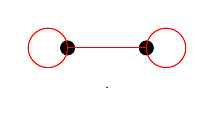
\begin{tikzpicture}[scale=0.5]
  \filldraw [black] (-1,0) circle (5pt);
  \filldraw [black] (1,0) circle (5pt);
  \draw[red] (-1,0) -- (1,0);
  \draw[red] (-1.5,0) circle (0.5);
  \draw[red] (1.5,0) circle (0.5);
  \filldraw [black] (0,-1) circle (0.01pt);
  \end{tikzpicture}
  \captionsetup{justification=centering}
  \caption{}
  \label{base case 3}
  \end{subfigure}
  \begin{subfigure}[b]{0.3\textwidth}
  \centering
  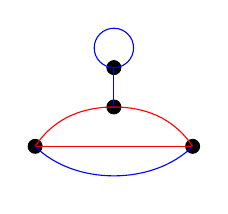
\begin{tikzpicture}[scale=0.5]
  \filldraw [black] (-2,0) circle (5pt);
  \filldraw [black] (2,0) circle (5pt);
  \filldraw[black] (0,1) circle (5pt);
  \filldraw (0,2) circle (5pt);
  \draw[red] (-2,0) -- (2,0);
  \draw[red] (-2,0) .. controls (-1.5,0.75) and (-0.75,1) .. (0,1);
  \draw[red] (2,0) .. controls (1.5,0.75) and (0.75,1) .. (0,1);
  \draw[blue] (-2,0) .. controls (-1,-1) and (1,-1) .. (2,0);
  \draw[blue] (0,1) -- (0,2);
  \draw[blue] (0,2.5) circle (0.5);
  \end{tikzpicture}
  \captionsetup{justification=centering}
  \caption{}
  \label{base case 4}
  \end{subfigure}
  \begin{subfigure}[b]{0.3\textwidth}
  \centering
  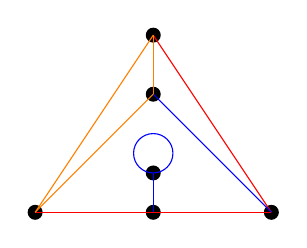
\begin{tikzpicture}[scale=0.5]
  \filldraw [black] (-3,0) circle (5pt);
  \filldraw [black] (3,0) circle (5pt);
  \filldraw[black] (0,1) circle (5pt);
  \filldraw (0,0) circle (5pt);
  \filldraw (0,3) circle (5pt);
  \filldraw (0,4.5) circle (5pt);
  \draw[red] (-3,0) -- (3,0);
  \draw[red] (3,0) -- (0,4.5);
  \draw[blue] (0,1.5) circle (0.5);
  \draw[blue] (0,0) -- (0,1);
  \draw[blue] (3,0) -- (0,3);
  \draw[orange] (-3,0) -- (0,3);)
  \draw[orange] (0,3) -- (0,4.5);
  \draw[orange] (-3,0) -- (0,4.5);
  \end{tikzpicture}
  \captionsetup{justification=centering}
  \caption{}
  \label{base case 5}
  \end{subfigure}
    \begin{subfigure}[b]{0.3\textwidth}
  \centering
  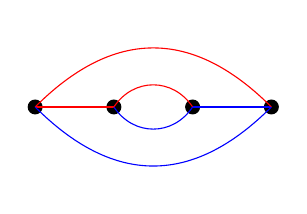
\begin{tikzpicture}[scale=0.5]
  \filldraw [black] (-3,0) circle (5pt);
  \filldraw [black] (-1,0) circle (5pt);
  \filldraw [black] (1,0) circle (5pt);
  \filldraw [black] (3,0) circle (5pt);
  \draw[red] (-3,0) -- (-1,0);
  \draw[red] (-1,0) .. controls (-0.5,0.75) and (0.5,0.75) .. (1,0);
  \draw[blue] (-1,0) .. controls (-0.5,-0.75) and (0.5,-0.75) .. (1,0);
  \draw[blue] (1,0) -- (3,0);
  \draw[red] (-3,0) .. controls (-1,2) and (1,2) .. (3,0);
  \draw[blue] (-3,0) .. controls (-1,-2) and (1,-2) .. (3,0);
  \end{tikzpicture}
  \captionsetup{justification=centering}
  \caption{}
  \label{base case 1}
  \end{subfigure}
  \begin{subfigure}[b]{0.3\textwidth}
  \centering
  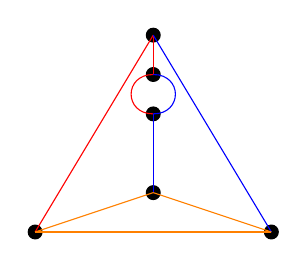
\begin{tikzpicture}[scale=0.5]
  \filldraw [black] (0,0) circle (5pt);
  \filldraw [black] (-3,-1) circle (5pt);
  \filldraw [black] (3,-1) circle (5pt);
  \filldraw [black] (0,2) circle (5pt);
  \filldraw [black] (0,3) circle (5pt);
  \filldraw [black] (0,4) circle (5pt);
  \draw[red] (-3,-1) -- (0,4);
  \draw[red] (0,4) -- (0,3);
  \draw[red] (0,2) .. controls (-0.75,2) and (-0.75,3) .. (0,3);
  \draw[blue] (0,2) .. controls (0.75,2) and (0.75,3) .. (0,3);
  \draw[blue] (0,0) -- (0,2);
  \draw[blue] (0,4) -- (3,-1);
  \draw[orange] (-3,-1) -- (3,-1);
  \draw[orange] (-3,-1) -- (0,0);
  \draw[orange] (3,-1) -- (0,0);
  \end{tikzpicture}
  \captionsetup{justification=centering}
  \caption{}
  \label{base case 2}
  \end{subfigure}
  \begin{subfigure}[b]{0.3\textwidth}
  \centering
  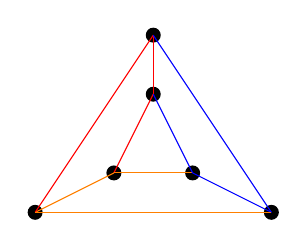
\begin{tikzpicture}[scale=0.5]
  \filldraw [black] (0,1) circle (5pt);
  \filldraw [black] (-1,-1) circle (5pt);
  \filldraw [black] (1,-1) circle (5pt);
  \filldraw [black] (0,2.5) circle (5pt);
  \filldraw [black] (-3,-2) circle (5pt);
  \filldraw [black] (3,-2) circle (5pt);
  \draw[red] (0,1) -- (-1,-1);
  \draw[orange] (-1,-1) -- (1,-1);
  \draw[blue] (1,-1) -- (0,1);
  \draw[red] (0,1) -- (0,2.5);
  \draw[orange] (-1,-1) -- (-3,-2);
  \draw[blue] (1,-1) -- (3,-2);
  \draw[red] (-3,-2) -- (0,2.5);
  \draw[blue] (3,-2) -- (0,2.5);
  \draw[orange] (-3,-2) -- (3,-2);
  \end{tikzpicture}
  \captionsetup{justification=centering}
  \caption{}
  \label{base case 6}
  \end{subfigure}
  \begin{subfigure}[b]{0.3\textwidth}
  \centering
  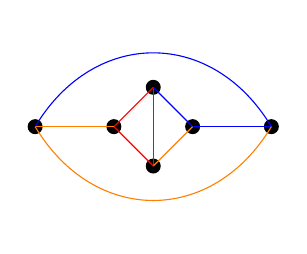
\begin{tikzpicture}[scale=0.5]
  \filldraw [black] (0,1) circle (5pt);
  \filldraw [black] (0,-1) circle (5pt);
  \filldraw [black] (1,0) circle (5pt);
  \filldraw [black] (-1,0) circle (5pt);
  \filldraw [black] (3,0) circle (5pt);
  \filldraw [black] (-3,0) circle (5pt);
  \draw[red] (0,1) -- (0,-1);
  \draw[blue] (0,1) -- (1,0);
  \draw[orange] (1,0) -- (0,-1);
  \draw[red] (0,-1) -- (-1,0);
  \draw[red] (-1,0) -- (0,1);
  \draw[blue] (1,0) -- (3,0);
  \draw[orange] (-1,0) -- (-3,0);
  \draw[blue] (-3,0) .. controls (-1.5,2.5) and (1.5,2.5) .. (3,0);
  \draw[orange] (-3,0) .. controls (-1.5,-2.5) and (1.5,-2.5) .. (3,0);
  \end{tikzpicture}
  \captionsetup{justification=centering}
  \caption{}
  \label{base case 7}
  \end{subfigure}
  \begin{subfigure}[b]{0.3\textwidth}
  \centering
  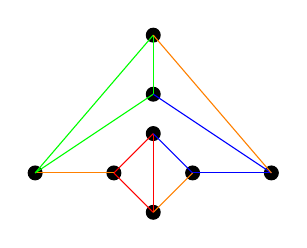
\begin{tikzpicture}[scale=0.5]
  \filldraw [black] (0,1) circle (5pt);
  \filldraw [black] (0,-1) circle (5pt);
  \filldraw [black] (1,0) circle (5pt);
  \filldraw [black] (-1,0) circle (5pt);
  \filldraw [black] (3,0) circle (5pt);
  \filldraw [black] (-3,0) circle (5pt);
  \filldraw (0,2) circle (5pt);
  \filldraw (0,3.5) circle (5pt);
  \draw[red] (0,1) -- (0,-1);
  \draw[blue] (0,1) -- (1,0);
  \draw[orange] (1,0) -- (0,-1);
  \draw[red] (0,-1) -- (-1,0);
  \draw[red] (-1,0) -- (0,1);
  \draw[blue] (1,0) -- (3,0);
  \draw[orange] (-1,0) -- (-3,0);
  \draw[green] (-3,0) -- (0,2);
  \draw[blue] (3,0) -- (0,2);
  \draw[green] (0,2) -- (0,3.5);
  \draw[green] (-3,0) -- (0,3.5);
  \draw[orange] (3,0) -- (0,3.5);
  \end{tikzpicture}
  \captionsetup{justification=centering}
  \caption{}
  \label{base case 8}
  \end{subfigure}
  \captionsetup{justification=centering}
  \caption{Base cases in the proof of Theorem~\ref{thm:P3EM}}
  \label{base case}
\end{figure}






\begin{proof}
By Lemma~\ref{lem:P3EM-equivalce}, it suffices to prove the case when $G$ is connected, as putting together P3EMs for each connected component gives a P3EM for $G$.

We  prove Theorem~\ref{thm:P3EM} by induction.
Our induction hypothesis is as follows: if $|V(G)| \le k$ for some integer $k$ and it is not one of the two exceptions, then it admits a P3EM. 
Given a larger graph $G$, 
we try to reduce it to a smaller graph $G'$ such that we obtain
a P3EM for $G$ from that of $G'$;
whenever the reduction step produces one of
the two exceptions, we will give a P3EM directly to the original graph.


\begin{figure}[ht]
  \centering
  \begin{subfigure}[b]{0.4\textwidth}
  \centering
  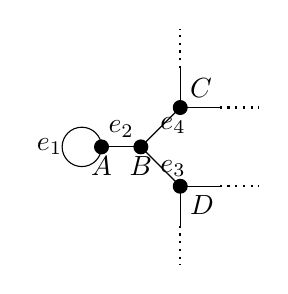
\begin{tikzpicture}[scale=0.5]
  \filldraw [black] (0,0) circle (5pt);
  \node[below] at (0,0) {$A$};
  \filldraw [black] (1,0) circle (5pt);
  \node[below] at (1,0) {$B$};
  \filldraw [black] (2,1) circle (5pt);
  \node[above right] at (2,1) {$C$};
  \filldraw [black] (2,-1) circle (5pt);
  \node[below right] at (2,-1) {$D$};
  \draw (-0.5,0) circle (0.5);
  \draw (0,0) -- (1,0);
  \draw (1,0) -- (2,1);
  \draw (1,0) -- (2,-1);
  \draw (2,1) -- (2,2);
  \draw (2,1) -- (3,1);
  \draw (2,-1) -- (3,-1);
  \draw (2,-1) -- (2,-2);
  \draw[thick, dotted] (2,2) -- (2,3);
  \draw[thick, dotted] (3,1) -- (4,1);
  \draw[thick, dotted] (3,-1) -- (4,-1);
  \draw[thick, dotted] (2,-2) -- (2,-3);
  \node[left] at (-0.75,0) {$e_1$};
  \node[above] at (0.5,0) {$e_2$};
  \node[below right] at (1.25,1) {$e_4$};
  \node[above right] at (1.25,-1) {$e_3$};
  \end{tikzpicture}
  \captionsetup{justification=centering}
  \caption{self loop in the original graph}
  \end{subfigure}
  \begin{subfigure}[b]{0.4\textwidth}
  \centering
  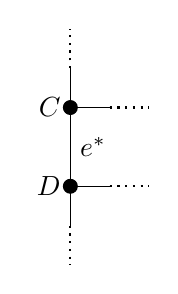
\begin{tikzpicture}[scale=0.5]
  \filldraw [black] (0,1) circle (5pt);
  \node[left] at (0,1) {$C$};
  \filldraw [black] (0,-1) circle (5pt);
  \node[left] at (0,-1) {$D$};
  \draw (0,1) -- (0,-1);
  \draw (0,1) -- (1,1);
  \draw (0,1) -- (0,2);
  \draw (0,-1) -- (0,-2);
  \draw (0,-1) -- (1,-1);
  \draw[thick, dotted] (0,2) -- (0,3);
  \draw[thick, dotted] (1,1) -- (2,1);
  \draw[thick, dotted] (0,-2) -- (0,-3);
  \draw[thick, dotted] (1,-1) -- (2,-1);
  \node[right] at (0,0) {$e^*$};
  \end{tikzpicture}
  \captionsetup{justification=centering}
  \caption{resulting graph}
  \end{subfigure}
  \captionsetup{justification=centering}
  \caption{Transforming self-loops}
  \label{self loop}
\end{figure}


We first show it suffices to consider simple planar 3-regular graphs.

 If $G$ has a self-loop, then locally it has a fragment depicted in Figure~\ref{self loop}, unless it is 
 planarly isomorphic to the base case Figure~\ref{base case 3}, which we
 directly give a P3EM. Now perform the transformation depicted in Figure~\ref{self loop}. If the resulting graph is one of the two exceptions, then the original graph is planarly isomorphic to the base cases Figure~\ref{base case 4} or Figure~\ref{base case 5}, for which we give their P3EMs directly. 
 %%%Note: there is no difference in which face the loop is placed , as on S^2, for both two exception graphs, all faces are equivalent.
 Otherwise, by induction hypothesis, there exists a P3EM $M$ for the resulting graph. If the edge $e^*$ in Figure~\ref{self loop}b is mapped rightwards ({\it resp.} leftwards) in $M$, then we obtain a P3EM for the original graph by simulating $e_4$ as $e^*$ to be mapped rightwards ({\it resp.} leftwards) and connecting $e_1$, $e_2$ and $e_3$.
Note that the self-loop transformation is valid regardless whether there is a self-loop at the vertices $C$ or $D$.

\begin{figure}[ht]
  \centering
  \begin{subfigure}[b]{0.4\textwidth}
  \centering
  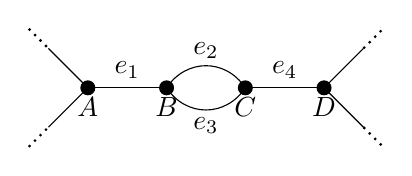
\begin{tikzpicture}[scale=0.5]
  \draw[thick, dotted] (-4.5,1.5) -- (-4,1);
  \draw[thick, dotted] (-4.5,-1.5) -- (-4,-1);
  \draw (-4,1) -- (-3,0);
  \draw (-4,-1) -- (-3,0);
  \filldraw [black] (-3,0) circle (5pt);
  \node[below] at (-3,0) {$A$};
  \draw (-3,0) -- (-1,0);
  \node[above] at (-2,0) {$e_1$};
  \filldraw [black] (-1,0) circle (5pt);
  \node[below] at (-1,0) {$B$};
  \draw (-1,0) .. controls (-0.5,0.75) and (0.5,0.75) .. (1,0);
  \node[above] at (0,0.5) {$e_2$};
  \draw (-1,0) .. controls (-0.5,-0.75) and (0.5,-0.75) .. (1,0);
  \node[below] at (0,-0.5) {$e_3$};
  \filldraw [black] (1,0) circle (5pt);
  \node[below] at (1,0) {$C$};
  \draw (1,0) -- (3,0);
  \node[above] at (2,0) {$e_4$};
  \filldraw [black] (3,0) circle (5pt);
  \node[below] at (3,0) {$D$};
  \draw (3,0) -- (4,1);
  \draw (3,0) -- (4,-1);
  \draw[thick, dotted] (4,1) -- (4.5,1.5);
  \draw[thick, dotted] (4,-1) -- (4.5,-1.5);
  \end{tikzpicture}
  \captionsetup{justification=centering}
  \caption{double edges in the original graph}
  \end{subfigure}
  \begin{subfigure}[b]{0.4\textwidth}
  \centering
  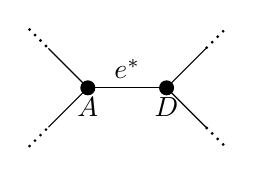
\begin{tikzpicture}[scale=0.5]
  \draw[thick, dotted] (-2.5,1.5) -- (-2,1);
  \draw[thick, dotted] (-2.5,-1.5) -- (-2,-1);
  \draw (-2,1) -- (-1,0);
  \draw (-2,-1) -- (-1,0);
  \filldraw [black] (-1,0) circle (5pt);
  \node[below] at (-1,0) {$A$};
  \draw (-1,0) -- (1,0);
  \node[above] at (0,0) {$e^*$};
  \filldraw [black] (1,0) circle (5pt);
  \node[below] at (1,0) {$D$};
  \draw (1,0) -- (2,1);
  \draw (1,0) -- (2,-1);
  \draw[thick, dotted] (2,1) -- (2.5,1.5);
  \draw[thick, dotted] (2,-1) -- (2.5,-1.5);
  \end{tikzpicture}
  \captionsetup{justification=centering}
  \caption{resulting graph}
  \end{subfigure}
  \captionsetup{justification=centering}
  \caption{Transforming double edges}
  \label{double edge}
\end{figure}


If $G$ has parallel edges between two vertices, say $B$ and $C$,
since  $G$ is 3-regular and 
$G$ is not planarly isomorphic to  $M_{2,3}$,
there must be exactly two edges between them.
If $B$ and $C$ have a common neighbor, say $A$, we may delete $B, C$ and their
incident edges, and add a self-loop at $A$. The resulting
graph is not one of the exceptions, by induction, it has a P3EM. One can then easily
obtain a P3EM for $G$.  
% form triple AB, AC, e_3 as in fig 3a, imagine Ab, AC from A below. then e2 simulates the loop at A
Now suppose the third edges from $B$ and $C$ are $e_1= \{A,B\}$ and $e_4 =\{C, D\}$
with $A \ne D$, as depicted in Figure~\ref{double edge}.
We likewise perform a transformation which ``deletes" $B$ and $C$  with double edges, 
and merge $e_1$ and $e_4$ to a single edge $e^* = \{A, D\}$.  If the resulting graph is one of the two exceptions, the original graph is isomorphic to the base cases Figure~\ref{base case 1} or Figure~\ref{base case 2} which we give their P3EMs directly. Otherwise, by induction hypothesis, there exists a P3EM $M$ for the resulting graph. If the edge $e^*$ is mapped upward ({\it resp.} downward) in $M$ (Figure~\ref{double edge}b), then we obtain a P3EM for the original graph by simulating $e_2$ ({\it resp.} $e_3$) as $e^*$ and connecting $e_3$ ({\it resp.} $e_2$), $e_1$ and $e_4$. 

Below we assume  $G$ is simple, i.e.,\ without parallel edges or self-loops.



\begin{figure}[ht]
  \centering
  \begin{subfigure}[b]{0.4\textwidth}
  \centering
  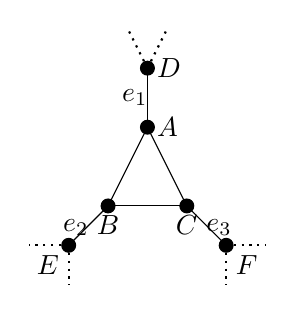
\begin{tikzpicture}[scale=0.5]
  \filldraw [black] (0,1) circle (5pt);
  \node[right] at (0,1) {$A$};
  \filldraw [black] (-1,-1) circle (5pt);
  \node[below] at (-1,-1) {$B$};
  \filldraw [black] (1,-1) circle (5pt);
  \node[below] at (1,-1) {$C$};
  \filldraw [black] (0,2.5) circle (5pt);
  \node[right] at (0,2.5) {$D$};
  \filldraw [black] (-2,-2) circle (5pt);
  \node[below left] at (-2,-2) {$E$};
  \filldraw [black] (2,-2) circle (5pt);
  \node[below right] at (2,-2) {$F$};
  \draw (0,1) -- (-1,-1);
  \draw (-1,-1) -- (1,-1);
  \draw (1,-1) -- (0,1);
  \draw (0,1) -- (0,2.5);
  \draw (-1,-1) -- (-2,-2);
  \draw (1,-1) -- (2,-2);
  \draw[thick, dotted] (-2,-2) -- (-3,-2);
  \draw[thick, dotted] (-2,-2) -- (-2,-3);
  \draw[thick, dotted] (2,-2) -- (3,-2);
  \draw[thick, dotted] (2,-2) -- (2,-3);
  \draw[thick, dotted] (0,2.5) -- (-0.5, 3.5);
  \draw[thick, dotted] (0,2.5) -- (0.5, 3.5);
  \node[left] at (0.25,1.75) {$e_1$};
  \node[above left] at (-1.25,-2) {$e_2$};
  \node[above right] at (1.25, -2) {$e_3$};
  \end{tikzpicture}
  \captionsetup{justification=centering}
  \caption{triangle in the original graph}
  \label{triangle 1}
  \end{subfigure}
  \begin{subfigure}[b]{0.4\textwidth}
  \centering
  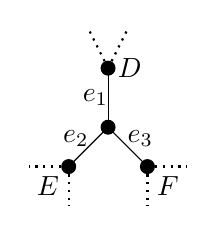
\begin{tikzpicture}[scale=0.5]
  \filldraw [black] (0,0) circle (5pt);
  \filldraw [black] (0,1.5) circle (5pt);
  \node[right] at (0,1.5) {$D$};
  \filldraw [black] (-1,-1) circle (5pt);
  \node[below left] at (-1,-1) {$E$};
  \filldraw [black] (1,-1) circle (5pt);
  \node[below right] at (1,-1) {$F$};
  \draw (0,0) -- (0,1.5);
  \draw (0,0) -- (-1,-1);
  \draw (0,0) -- (1,-1);
  \draw[thick, dotted] (0,1.5) -- (-0.5,2.5);
  \draw[thick, dotted] (0,1.5) -- (0.5,2.5);
  \draw[thick, dotted] (-1,-1) -- (-2,-1);
  \draw[thick, dotted] (-1,-1) -- (-1,-2);
  \draw[thick, dotted] (1,-1) -- (2,-1);
  \draw[thick, dotted] (1,-1) -- (1,-2);
  \node[left] at (0.25, 0.75) {$e_1$};
  \node[above left] at (-0.25,-0.75) {$e_2$};
  \node[above right] at (0.25,-0.75) {$e_3$};
  \end{tikzpicture}
  \captionsetup{justification=centering}
  \caption{resulting graph}
  \label{triangle 2}
  \end{subfigure}
  \\
  \begin{subfigure}[b]{0.4\textwidth}
  \centering
  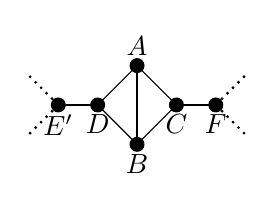
\begin{tikzpicture}[scale=0.5]
  \filldraw [black] (0,1) circle (5pt);
  \node[above] at (0,1) {$A$};
  \filldraw [black] (0,-1) circle (5pt);
  \node[below] at (0,-1) {$B$};
  \filldraw [black] (1,0) circle (5pt);
  \node[below] at (1,0) {$C$};
  \filldraw [black] (-1,0) circle (5pt);
  \node[below] at (-1,0) {$D$};
  \filldraw [black] (2,0) circle (5pt);
  \node[below] at (2,0) {$F$};
  \filldraw [black] (-2,0) circle (5pt);
  \node[below] at (-2,0) {$E'$};
  \draw (0,1) -- (0,-1);
  \draw (0,1) -- (1,0);
  \draw (1,0) -- (0,-1);
  \draw (0,-1) -- (-1,0);
  \draw (-1,0) -- (0,1);
  \draw (1,0) -- (2,0);
  \draw (-1,0) -- (-2,0);
  \draw[thick, dotted] (2,0) -- (2.75,0.75);
  \draw[thick, dotted] (2,0) -- (2.75,-0.75);
  \draw[thick, dotted] (-2,0) -- (-2.75, 0.75);
  \draw[thick, dotted] (-2,0) -- (-2.75, -0.75);
  \end{tikzpicture}
  \captionsetup{justification=centering}
  \caption{triangle in the original graph ($D=E$)}
  \label{triangle 3}
  \end{subfigure}
  \begin{subfigure}[b]{0.4\textwidth}
  \centering
  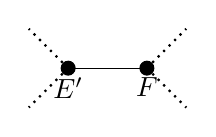
\begin{tikzpicture}[scale=0.5]
  \filldraw [black] (1,0) circle (5pt);
  \node[below] at (1,0) {$F$};
  \filldraw [black] (-1,0) circle (5pt);
  \node[below] at (-1,0) {$E'$};
  \draw (-1,0) -- (1,0);
  \draw[thick, dotted] (1,0) -- (2,1);
  \draw[thick, dotted] (1,0) -- (2,-1);
  \draw[thick, dotted] (-1,0) -- (-2,1);
  \draw[thick, dotted] (-1,0) -- (-2,-1);
  \end{tikzpicture}
  \captionsetup{justification=centering}
  \caption{resulting graph ($D=E$)}
  \label{triangle 4}
  \end{subfigure}
  \captionsetup{justification=centering}
  \caption{Transforming triangles}
  \label{triangle}
\end{figure}


Next we consider the case when $G$ contains 
a triangle face as depicted in  Figure~\ref{triangle 1}. Since it is a simple graph, all three edges $e_1, e_2, e_3$ are distinct, and
$D, E, F \not \in \{A, B, C\}$. If the vertices $D, E, F$ are all distinct,  then we perform the transformation from Figure~\ref{triangle 1} to Figure~\ref{triangle 2}. By induction hypothesis, the resulting graph admits a P3EM unless it is $K_4$ (in this case, the resulting graph cannot be $M_{2,3}$ since it has more than two vertices). If the resulting graph is $K_4$, then the original graph is (or planarly isomorphic to)
the base case Figure~\ref{base case 6} for which we give a P3EM directly. If the resulting graph is not $K_4$ and hence admits a P3EM $M$ by our induction hypothesis, then the original graph can simulate $M$ by connecting the edges of the triangle face internally. We now consider the case when the vertices $D,E,F$ are not all distinct. Since the original graph is not $K_4$,  the vertices $D,E,F$ are not all the same vertex. Without loss of generality we assume $D=E\neq F$. See Figure~\ref{triangle 3} for an illustration. 
$D$ has an incident vertex $E' \ne A, B$.  Suppose $E' \ne F$. Then we perform the transformation illustrated in Figure~\ref{triangle 4}. Similarly as above, if the resulting graph is not one of the exceptions, then we can easily simulate the P3EM (which is given by the induction) in the resulting graph.
%%%internally form triple AB BC CA.  use AD to simulate E'F. if E'F goes up, then below in the Fig 4c form triple E'D, DB, CF.
If the resulting graph Figure~\ref{triangle 4} is planarly isomorphic to the exceptions $M_{2,3}$ or $K_4$, then the original graph is planarly isomorphic to the base cases Figure~\ref{base case 7} or Figure~\ref{base case 8}, which we give a P3EM directly. Finally suppose $E'=F$, then we transform the original graph by deleting  the vertices  $A, B, C, D$ 
and their incident edges, and form a self-loop at $E'= F$. The resulting graph has fewer vertices
(and has a self-loop and so it is not $M_{2,3}$ or $K_4$), and so
by the induction hypothesis 
 it admits a P3EM. It is easy to verify that a P3EM in the resulting graph, as before, can be simulated in the original graph. 
 %%% any P3EM in G' assigns loop outward.
 %%% assign ABC. use AD simulate the loop. internally form E'D, DB, E'C
In the following we may  assume $G$ is simple without triangle faces. 


\begin{figure}[ht]
  \centering
  \begin{subfigure}[b]{0.4\textwidth}
  \centering
  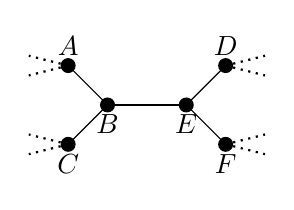
\begin{tikzpicture}[scale=0.5]
  \filldraw [black] (-1,0) circle (5pt);
  \node[below] at (-1,0) {$B$};
  \filldraw [black] (-2,1) circle (5pt);
  \node[above] at (-2,1) {$A$};
  \filldraw [black] (-2,-1) circle (5pt);
  \node[below] at (-2,-1) {$C$};
  \filldraw [black] (1,0) circle (5pt);
  \node[below] at (1,0) {$E$};
  \filldraw [black] (2,1) circle (5pt);
  \node[above] at (2,1) {$D$};
  \filldraw [black] (2,-1) circle (5pt);
  \node[below] at (2,-1) {$F$};
  \draw (-1,0) -- (1,0);
  \draw (-1,0) -- (-2,1);
  \draw (-1,0) -- (-2,-1);
  \draw (1,0) -- (2,1);
  \draw (1,0) -- (2,-1);
  \draw[thick, dotted] (-2,1) -- (-3,1.25);
  \draw[thick, dotted] (-2,1) -- (-3,0.75);
  \draw[thick, dotted] (-2,-1) -- (-3, -1.25);
  \draw[thick, dotted] (-2,-1) -- (-3,-0.75);
  \draw[thick, dotted] (2,1) -- (3,1.25);
  \draw[thick, dotted] (2,1) -- (3,0.75);
  \draw[thick, dotted] (2,-1) -- (3,-0.75);
  \draw[thick, dotted] (2,-1) -- (3,-1.25);
  \end{tikzpicture}
  \captionsetup{justification=centering}
  \caption{bridge in the original graph}
  \end{subfigure}
  \begin{subfigure}[b]{0.4\textwidth}
  \centering
  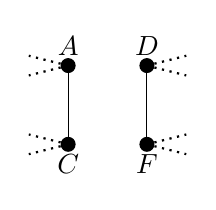
\begin{tikzpicture}[scale=0.5]
  \filldraw [black] (-1,1) circle (5pt);
  \node[above] at (-1,1) {$A$};
  \filldraw [black] (-1,-1) circle (5pt);
  \node[below] at (-1,-1) {$C$};
  \filldraw [black] (1,1) circle (5pt);
  \node[above] at (1,1) {$D$};
  \filldraw [black] (1,-1) circle (5pt);
  \node[below] at (1,-1) {$F$};
  \draw (-1,-1) -- (-1,1);
  \draw (1,1) -- (1,-1);
  \draw[thick, dotted] (-1,1) -- (-2, 1.25);
  \draw[thick, dotted] (-1,1) -- (-2,0.75);
  \draw[thick, dotted] (-1,-1) -- (-2, -0.75);
  \draw[thick, dotted] (-1,-1) -- (-2, -1.25);
  \draw[thick, dotted] (1,1) -- (2,1.25);
  \draw[thick, dotted] (1,1) -- (2,0.75);
  \draw[thick, dotted] (1,-1) -- (2,-0.75);
  \draw[thick, dotted] (1,-1) -- (2,-1.25);
  \end{tikzpicture}
  \captionsetup{justification=centering}
  \caption{resulting graph}
  \end{subfigure}
  \captionsetup{justification=centering}
  \caption{Transforming a bridge}
  \label{bridge}
\end{figure}




Next we consider the case when the graph contains a  bridge, i.e.,
an edge whose removal disconnects the graph (see Figure~\ref{bridge}a). 
%We show that if $G$ has a bridge then it admits a P3EM.
This means that the same face $f$  is on both sides of the bridge
$\{B,E\}$ in $G$. 
Perform the transformation illustrated in Figure~\ref{bridge}. The resulting graph has two disconnected components which are not isomorphic to any exception case. Indeed, neither is isomorphic to $M_{2,3}$ since $G$ has no
parallel edges, and if it were
$K_4$ then the original graph $G$ contains a triangle face. 
Thus by induction there are P3EMs, $M_1$ and $M_2$, for the two components respectively. We will use the  edges $\{B,C\}$ and $\{E,F\}$ 
to simulate $\{A,C\}$ and $\{D,F\}$ respectively, and  match
the three edges $\{A,B\}, \{B,E\}$ and $\{E,D\}$ directly. Then we obtain a
P3EM for $G$ from $M_1$ and $M_2$. 
Note that
both $\{B,C\}$ and $\{E,F\}$ are on the face $f$.
Since  $\{B, E\}$ is a bridge, regardless of how  $\{A,C\}$ and $\{D,F\}$ are matched respectively by $M_1$ and $M_2$,
we can substitute $\{B,C\}$ and $\{E,F\}$ for them respectively.
When viewed in a spherical
embedding, we may assume both  $\{A,C\}$ and $\{D,F\}$ are on the outer face
for the two disconnected components. 
 Then  in $G$ the substitution of   $\{B,C\}$ for $\{A,C\}$,
 and  $\{E,F\}$ 
for $\{D,F\}$, gives 
 a total number of edges assigned to the face $f$ in $G$
to be the sum of the corresponding numbers assigned by $M_1$ and $M_2$, and thus this total number is 
$\equiv 0 \pmod{3} $. Below we assume the graph has no bridges.



\begin{figure}[ht]
  \centering
  \begin{subfigure}[b]{0.4\textwidth}
  \centering
  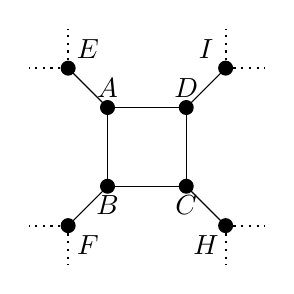
\begin{tikzpicture}[scale=0.5]
  \filldraw [black] (-1,1) circle (5pt);
  \node[above] at (-1,1) {$A$};
  \filldraw [black] (-1,-1) circle (5pt);
  \node[below] at (-1,-1) {$B$};
  \filldraw [black] (1,-1) circle (5pt);
  \node[below] at (1,-1) {$C$};  
  \filldraw [black] (1,1) circle (5pt);
  \node[above] at (1,1) {$D$};
  \filldraw [black] (-2,2) circle (5pt);
  \node[above] at (-1.5,2) {$E$};
  \filldraw [black] (-2,-2) circle (5pt);
  \node[below] at (-1.5,-2) {$F$};
  \filldraw [black] (2,-2) circle (5pt);
  \node[below] at (1.5,-2) {$H$};
  \filldraw [black] (2,2) circle (5pt);
  \node[above] at (1.5,2) {$I$};
  \draw (-1,1) -- (-1,-1);
  \draw (-1,-1) -- (1,-1);
  \draw (1,-1) -- (1,1);
  \draw (1,1) -- (-1,1);
  \draw (-1,1) -- (-2,2);
  \draw (-1,-1) -- (-2,-2);
  \draw (1,-1) -- (2,-2);
  \draw (1,1) -- (2,2);
  \draw[thick, dotted] (-2,2) -- (-3,2);
  \draw[thick, dotted] (-2,2) -- (-2,3);
  \draw[thick, dotted] (-2,-2) -- (-3,-2);
  \draw[thick, dotted] (-2,-2) -- (-2,-3);
  \draw[thick, dotted] (2,-2) -- (3,-2);
  \draw[thick, dotted] (2,-2) -- (2,-3);
  \draw[thick, dotted] (2,2) -- (3,2);
  \draw[thick, dotted] (2,2) -- (2,3);
  \end{tikzpicture}
  \captionsetup{justification=centering}
  \caption{square in the original graph}
  \end{subfigure}
  \begin{subfigure}[b]{0.4\textwidth}
  \centering
  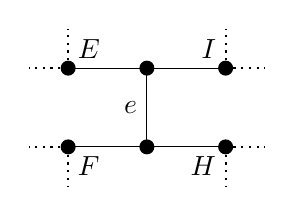
\begin{tikzpicture}[scale=0.5]
  \filldraw [black] (0,1) circle (5pt);
  \filldraw [black] (0,-1) circle (5pt);
  \filldraw [black] (2,1) circle (5pt);
  \node[above left] at (2,1) {$I$};
  \filldraw [black] (2,-1) circle (5pt);
  \node[below left] at (2,-1) {$H$};
  \filldraw [black] (-2,1) circle (5pt);
  \node[above right] at (-2,1) {$E$};
  \filldraw [black] (-2,-1) circle (5pt);
  \node[below right] at (-2,-1) {$F$};
  \draw (-2,1) -- (2,1);
  \draw (-2,-1) -- (2,-1);
  \draw (0,1) -- (0,-1);
  \node[left] at (0,0) {$e$};
  \draw[thick, dotted] (-2,1) -- (-3,1);
  \draw[thick, dotted] (-2,1) -- (-2,2);
  \draw[thick, dotted] (-2,-1) -- (-3,-1);
  \draw[thick, dotted] (-2,-1) -- (-2,-2);
  \draw[thick, dotted] (2,1) -- (3,1);
  \draw[thick, dotted] (2,1) -- (2,2);
  \draw[thick, dotted] (2,-1) -- (3,-1);
  \draw[thick, dotted] (2,-1) -- (2,-2);
  \end{tikzpicture}
  \captionsetup{justification=centering}
  \caption{resulting graph}
  \end{subfigure}
  \captionsetup{justification=centering}
  \caption{Transforming a square}
  \label{square}
\end{figure}


We show next that if $G$ has a square face, then it admits a P3EM. 
See Figure~\ref{square} for an illustration. Since it is simple,
$E$ is distinct from $B, D$. Also $E \ne C$, for otherwise
$\{B, F\}$ or $\{D, I\}$ would be a bridge.
%%% suppose E=C. then in fact both would be bridges: doeen't matter which way 
% the edge AC winds around. We traverse Ab, BC, with square on Left, then CA
%% gets a cycle ABC. the part of G containing the equare is sepaeate from
% the part og G connected to B via BF.
% similarly, travers AD, DC, CA with sq on its right, gets cycle ADC , shows
% DI is bridge. 
By the same reason, none of the vertices $E, F, H, I$ can be from $\{A, B, C, D\}$.
If $E = H$ we again would have a bridge.
%%% this time we can only guarantee one bridge: E=H has one more edge going off. if goes outward, ie not in the face formed by the cycle ADCE, then DI is a bridge as ADCE with sq on R shows (all A, C, E can't have any more incident edges)
% if that edge from E=H goes inward, ie inside the part bounded by the cycle ADCE,
%then BF is a bridge, as cycle ABCE with sq on Left shows. 
Also $E \ne F, I$, because $G$ has no triangle face.
It follows that all $A, B, C, D, E, F, H, I$ are distinct.
Now we perform the transformation in Figure~\ref{square}, replacing the
square $ABCD$ by an edge $e$.  It is clearly not one of the exception graphs 
(it has  at least 6 vertices).
By induction hypothesis, the resulting graph admits a P3EM $M$. If $e$ in the resulting graph is mapped leftwards,
then  we can simulate $M$ in $G$ by mapping $\{A,B\}$ leftwards, and 
match $\{A,D\}$, $\{D,C\}$ and $\{C,B\}$ inside the square.
Similarly, if $e$  is mapped rightwards, then we use $\{D, C\}$ in its place,
and match $\{A,D\}$, $\{A, B\}$ and $\{B, C\}$ inside the square.
This gives a P3EM for $G$. Below we assume $G$ has no square faces.


\begin{figure}[ht]
  \centering
  \begin{subfigure}[b]{0.4\textwidth}
  \centering
  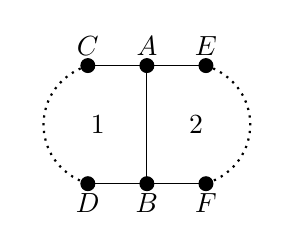
\begin{tikzpicture}[scale=0.5]
  \filldraw [black] (0,1.5) circle (5pt);
  \node[above] at (0,1.5) {$A$};
  \filldraw [black] (0,-1.5) circle (5pt);
  \node[below] at (0,-1.5) {$B$};
  %\filldraw [black] (-1,2) circle (5pt);
  %\node[above] at (-1,2) {$C$};
  \filldraw [black] (-1.5,1.5) circle (5pt);
  \node[above] at (-1.5,1.5) {$C$};
  %\filldraw [black] (-1,-2) circle (5pt);
  %\node[below] at (-1,-2) {$D$};
  \filldraw [black] (-1.5,-1.5) circle (5pt);
  \node[below] at (-1.5,-1.5) {$D$};
  %\filldraw [black] (1,2) circle (5pt);
  %\node[above] at (1,2) {$E$};
  \filldraw [black] (1.5,1.5) circle (5pt);
  \node[above] at (1.5,1.5) {$E$};
  %\filldraw [black] (1,-2) circle (5pt);
  %\node[below] at (1,-2) {$F$};
  \filldraw [black] (1.5,-1.5) circle (5pt);
  \node[below] at (1.5,-1.5) {$F$};
  \draw (0,1.5) -- (0,-1.5);
  \draw (0,1.5) -- (-1.5,1.5);
  \draw (0,1.5) -- (1.5,1.5);
  \draw (0,-1.5) -- (-1.5,-1.5);
  \draw (0,-1.5) -- (1.5, -1.5);
  \draw[thick, dotted] (-1.5,1.5) .. controls (-3,1) and (-3,-1) .. (-1.5,-1.5);
  \draw[thick, dotted] (1.5,1.5) .. controls (3,1) and (3,-1) .. (1.5,-1.5);
  \node at (-1.25,0) {$1$};
  \node at (1.25,0) {$2$};
  \end{tikzpicture}
  \captionsetup{justification=centering}
  \caption{chord in the original graph}
  \label{chord_1}
  \end{subfigure}
  \begin{subfigure}[b]{0.4\textwidth}
  \centering
  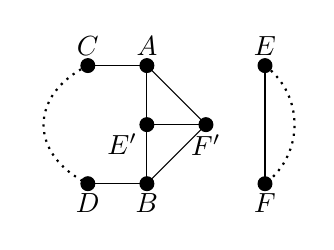
\begin{tikzpicture}[scale=0.5]
  \filldraw [black] (0,0) circle (5pt);
  \node[left] at (0,-0.5) {$E'$};
  \filldraw [black] (0,1.5) circle (5pt);
  \node[above] at (0,1.5) {$A$};
  \filldraw [black] (0,-1.5) circle (5pt);
  \node[below] at (0,-1.5) {$B$};
  \filldraw [black] (-1.5,1.5) circle (5pt);
  \node[above] at (-1.5,1.5) {$C$};
  \filldraw [black] (-1.5,-1.5) circle (5pt);
  \node[below] at (-1.5,-1.5) {$D$};
  \filldraw [black] (1.5,0) circle (5pt);
  \node[below] at (1.5,0) {$F'$};
  \filldraw [black] (3,-1.5) circle (5pt);
  \node[below] at (3,-1.5) {$F$};
  \filldraw [black] (3,1.5) circle (5pt);
  \node[above] at (3,1.5) {$E$};
  \draw (0,0) -- (0,1.5);
  \draw (0,0) -- (0,-1.5);
  \draw (0,1.5) -- (-1.5,1.5);
  \draw (0,-1.5) -- (-1.5,-1.5);
  \draw (0,-1.5) -- (1.5,0);
  \draw (0,0) -- (1.5, 0);
  \draw (0,1.5) -- (1.5,0);
  \draw[thick, dotted] (-1.5,1.5) .. controls (-3,0.75) and (-3,-0.75) .. (-1.5,-1.5);
  \draw (3,1.5) -- (3,-1.5);
  \draw[thick, dotted] (3,1.5) .. controls (4, 0.75) and (4,-0.75) .. (3,-1.5);
  \end{tikzpicture}
  \captionsetup{justification=centering}
  \caption{resulting graph}
  \end{subfigure}
  \captionsetup{justification=centering}
  \caption{Transforming a chord}
  \label{chord}
\end{figure}


We now consider the case when the graph contains a chord. Let $\mathcal{C}$ be the boundary of the external face of the plane graph. Since we can now assume $G$ is bridgeless, $\mathcal{C}$ is a simple cycle. We say it contains a chord  if there exist two vertices on $\mathcal{C}$ that are joined by an edge that is not in $\mathcal{C}$. See Figure~\ref{chord}a for an illustration. 
Since  $\mathcal{C}$  is the outer boundary,
any chord must connect inside of $\mathcal{C}$.
Let $\{A, B\}$ be a chord, and let $C, E$ and $D, F$ be their neighbors on $\mathcal{C}$.
We note that there is no edge connecting $\{C,D\}$ or $\{E,F\}$ since  $G$ has no square
face. In Figure~\ref{chord}a 
we mark the part of $G$ to the left, respectively to the right, of (but including) the edge $\{A,B\}$ 
as region 1, respectively  region 2. 
By planarity, the only edges connecting 
 regions 1 and  2 are those incident to $A$ or $B$. 
%and to the right of 
Denote the numbers of edges in regions 1 and 2 by $E_1$ and $E_2$
(both including $\{A,B\}$). Then $E_1 + E_2  \equiv 1 \pmod{3}$. Perform the transformation illustrated in Figure~\ref{chord} and we obtain a resulting graph that is disconnected and its two components are 3-regular plane graphs. Since in the original graph, $E$ and $F$ are not adjacent, there exists another vertex distinct from $E$ and $F$ in region 2. Thus, the left side component in the resulting graph has at least one vertex fewer than $G$, and by induction hypothesis it admits a P3EM $M'_1$. Similarly, the right side component also admits a P3EM $M'_2$ (it cannot be $M_{2,3}$ since $G$ is simple,
 nor  $K_4$ since that will imply $G$ has a triangle face). 
The edge $\{E',F'\}$ is 
assigned either inside the triangle $AE'F'$ or inside $BE'F'$.
In the former case, 
the edges $\{B, E'\}$ and $\{B, F'\}$ must be assigned outside the triangle $BE'F'$.
In the latter case,  the edges $\{A, E'\}$ and $\{A, F'\}$ are assigned outside the triangle $AE'F'$. In either case, exactly one of the edges $\{A, E'\}$ or $\{B, E'\}$ is assigned leftwards and one of the edges $\{A, F'\}$ or $\{B, F'\}$ is assigned outside. Thus, there are $N_1 \equiv 2 \pmod{3}$ edges in the path  $(A,C,\dots, D, B)$ along the cycle  $\mathcal{C}$ assigned outside. Similarly, let $N_2$ denote the number of edges assigned outside along the external face in $M'_2$, then $N_2 \equiv 0 \pmod{3}$.
We now construct a 3DEM in $G$. In region 1, the
edge $\{A,B\}$ will be assigned leftwards (taking its place as either
$\{A, E'\}$ or $\{B, E'\}$ which was assigned leftwards in $M'_1$).
All other edges will be assigned
in the same way as in $M'_1$. 
 In region 2 we assign all edges, other than $\{A,B\}$, as follows.
 The edge $\{B,F\}$ will be assigned outside (taking its place as either
 $\{A, F'\}$ or $\{B, F'\}$ which was assigned outside in $M'_1$);
 $\{A, E\}$ will be assigned as $\{E, F\}$ in $M'_2$;
all other edges 
will be assigned the same way as in $M'_2$. By doing so, all internal faces
are assigned  $0 \pmod{3}$ edges, as in the case of $M'_1$ and $M'_2$. For the external face, note that there are also $N_1 + 1 + N_2 \equiv 0 \pmod{3}$ edges assigned to it in total. Thus our construction gives a valid P3EM in $G$.


To summarize, we can assume now that the  3-regular plane graph $G$ is  simple, without triangle and square faces, bridgeless and  chordless. We now show that the graph must have a pentagon face. Let $v,e,f$ denote the number of vertices, edges and faces (including the external one) of $G$, respectively. Since $G$ is 3-regular, we have $3v=2e$. Suppose the minimum number of edges around any face is $n$, then $2e \geq nf$. 
By Euler's formula, we have $2 = v-e+f \le (2/n - 1/3) e$, and thus
$n < 6$. Since $G$ is simple and
without triangle and square faces, we have $n=5$.


\begin{figure}[ht]
  \centering
%  \begin{subfigure}[b]{0.4\textwidth}
%  \centering
  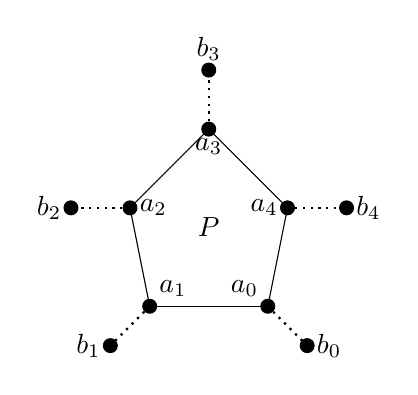
\begin{tikzpicture}[scale=0.5]
  \node at (0,0.5) {$P$};
  \filldraw [black] (1.5,-1.5) circle (5pt);
  \node[above left] at (1.5,-1.5) {$a_0$};
  \filldraw [black] (-1.5,-1.5) circle (5pt);
  \node[above right] at (-1.5,-1.5) {$a_1$};
  \filldraw [black] (-2,1) circle (5pt);
  \node[right] at (-2,1) {$a_2$};
  \filldraw [black] (2,1) circle (5pt);
  \node[left] at (2,1) {$a_4$};
  \filldraw [black] (0,3) circle (5pt);
  \node[below] at (0,3) {$a_3$};
  \filldraw [black] (2.5,-2.5) circle (5pt);
  \node[right] at (2.5,-2.5) {$b_0$};
  \filldraw [black] (-2.5,-2.5) circle (5pt);
  \node[left] at (-2.5,-2.5) {$b_1$};
  \filldraw [black] (-3.5,1) circle (5pt);
  \node[left] at (-3.5,1) {$b_2$};
  \filldraw [black] (3.5,1) circle (5pt);
  \node[right] at (3.5,1) {$b_4$};
  \filldraw [black] (0,4.5) circle (5pt);
  \node[above] at (0,4.5) {$b_3$};
  \draw (1.5,-1.5) -- (-1.5,-1.5);
  \draw (-1.5, -1.5) -- (-2,1);
  \draw (-2,1) -- (0,3);
  \draw (0,3) -- (2,1);
  \draw (2,1) -- (1.5,-1.5);
  \draw[thick, dotted] (1.5,-1.5) -- (2.5,-2.5);
  \draw[thick, dotted] (-1.5,-1.5) -- (-2.5,-2.5);
  \draw[thick, dotted] (0,3) -- (0,4.5);
  \draw[thick, dotted] (-2,1) -- (-3.5,1);
  \draw[thick, dotted] (2,1) -- (3.5,1);
  \end{tikzpicture}  
  \captionsetup{justification=centering}
   \caption{Pentagon in the original graph}
   \label{pentagon_path_1}
\end{figure}


Now fix a pentagon face $P$ in the graph
with vertices $\{a_0, a_1, \ldots, a_4\}$. See Figure~\ref{pentagon_path_1} for an illustration. Since $G$ is 3-regular, simple and bridgeless,
there is a neighbor
$b_i$   of $a_i$ distinct from $\{a_0, a_1, \ldots, a_4\}$, for every $0\le i \le 4$.
For example,  $b_0 \ne a_1$ by simplicity.
If $b_0=a_2$, i.e., if $\{a_0,a_2\}$ were an edge, then
there would be a bridge $\{a_1, b_1\}$.
Indeed, the edge $\{a_0,a_2\}$ must lie outside of the pentagon face $P$.
If one traverses the edges $\{a_2,a_1\}, \{a_1,a_0\}$ with $P$ to its left,
then follows with the edge $\{a_0,a_2\}$, one gets a cycle which separates the part
of $G$ that contains $P$ from the part of $G$ that connects to $a_1$ via the edge $\{a_1,b_1\}$ (note that all three neighbors of each vertex in $\{a_0,a_1,a_2\}$ are accounted for and thus no other adjacent edge exists to the right of this cycle). So,
deleting $\{a_1,b_1\}$  disconnects $G$, and thus
$\{a_1,b_1\}$  is a bridge. Thus, $b_0 \not =a_2$ as $G$ is bridgeless. See Figure~\ref{fig:b0neqa2} for an illustration.
By symmetry, $b_0 \ne a_3, a_4$ as well.
%and if $b_0$ were $a_2$ 
%there would be a bridge $\{a_1, b_1\}$.
By the same reason, 
$b_i \not \in \{a_0, a_1, \ldots, a_4\}$,
 for all $0\le i \le 4$.

 \begin{figure}[ht]
  \centering
  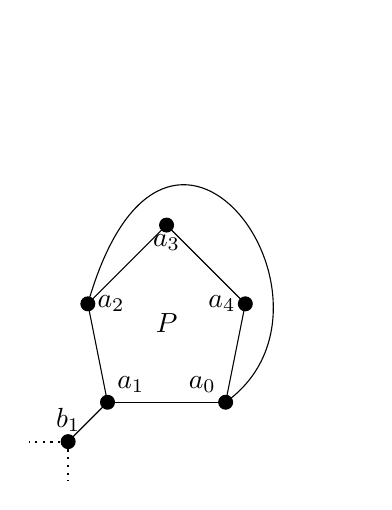
\begin{tikzpicture}[scale=0.5]
  \node at (0,0.5) {$P$};
  \filldraw [black] (1.5,-1.5) circle (5pt);
  \node[above left] at (1.5,-1.5) {$a_0$};
  \filldraw [black] (-1.5,-1.5) circle (5pt);
  \node[above right] at (-1.5,-1.5) {$a_1$};
  \filldraw [black] (-2,1) circle (5pt);
  \node[right] at (-2,1) {$a_2$};
  \filldraw [black] (2,1) circle (5pt);
  \node[left] at (2,1) {$a_4$};
  \filldraw [black] (0,3) circle (5pt);
  \node[below] at (0,3) {$a_3$};
  %\filldraw [black] (2.5,-2.5) circle (5pt);
  %\node[right] at (2.5,-2.5) {$b_0$};
  \filldraw [black] (-2.5,-2.5) circle (5pt);
  \node[above] at (-2.5,-2.5) {$b_1$};
  %\filldraw [black] (-3.5,1) circle (5pt);
  %\node[left] at (-3.5,1) {$b_2$};
  %\filldraw [black] (3.5,1) circle (5pt);
  %\node[right] at (3.5,1) {$b_4$};
  %\filldraw [black] (0,4.5) circle (5pt);
  %\node[above] at (0,4.5) {$b_3$};
  \draw (1.5,-1.5) -- (-1.5,-1.5);
  \draw (-1.5, -1.5) -- (-2,1);
  \draw (-2,1) -- (0,3);
  \draw (0,3) -- (2,1);
  \draw (2,1) -- (1.5,-1.5);
  %\draw[thick, dotted] (1.5,-1.5) -- (2.5,-2.5);
  \draw (-1.5,-1.5) -- (-2.5,-2.5);
  %\draw (0,3) -- (0,4.5);
  %\draw[thick, dotted] (-2,1) -- (-3.5,1);
  %\draw (2,1) -- (3.5,1);
  \draw[thick, dotted] (-2.5,-2.5) -- (-2.5,-3.5);
  \draw[thick, dotted] (-2.5,-2.5) -- (-3.5,-2.5);
  \draw (-2,1) .. controls (0,8) and (5,1) .. (1.5,-1.5);
  \end{tikzpicture}
  \captionsetup{justification=centering}
   \caption{Why $b_0 \neq a_2$}
   \label{fig:b0neqa2}
\end{figure}


Furthermore, since $G$ has no triangle or square
faces
 and is bridgeless, we claim that without loss of generality
$b_i$ are all distinct ($ 0 \le i\le 4$). To see that, we first note that
 $b_0 \ne b_1, b_4$, for otherwise
there would be a triangle face.
Next we deal with the case  $b_0 = b_2$ or $b_0 = b_3$.
By symmetry suppose $b_0 = b_2$. There is
a third adjacent vertex $b$ of $b_0$, other than $a_0, a_2$. Consider the
cycle $C = (a_2, a_1, a_0, b_0=b_2, a_2)$ with
$P$ to its left, which defines two simply connected
regions in the spherical embedding of $G$. Call the region that contains $P$
the  interior region. If the edge $\{b_0, b\}$
is in the interior region, then $\{a_1, b_1\}$
is a bridge, by the same proof for $b_0 \ne a_2$. So we may assume $\{b_0, b\}$
lies in the exterior region of  the cycle $C$. (See Figure~\ref{trouble}.)

\begin{figure}[ht]
  \centering
%  \begin{subfigure}[b]{0.4\textwidth}
%  \centering
  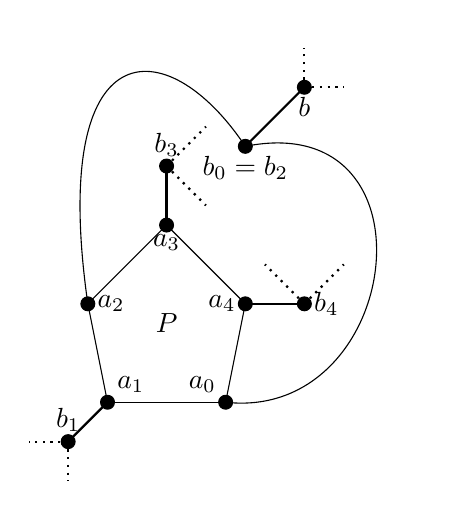
\begin{tikzpicture}[scale=0.5]
  \node at (0,0.5) {$P$};
  \filldraw [black] (1.5,-1.5) circle (5pt);
  \node[above left] at (1.5,-1.5) {$a_0$};
  \filldraw [black] (-1.5,-1.5) circle (5pt);
  \node[above right] at (-1.5,-1.5) {$a_1$};
  \filldraw [black] (-2,1) circle (5pt);
  \node[right] at (-2,1) {$a_2$};
  \filldraw [black] (2,1) circle (5pt);
  \node[left] at (2,1) {$a_4$};
  \filldraw [black] (0,3) circle (5pt);
  \node[below] at (0,3) {$a_3$};
  \filldraw [black] (-2.5,-2.5) circle (5pt);
  \node[above] at (-2.5,-2.5) {$b_1$};
  \filldraw [black] (3.5,1) circle (5pt);
  \node[right] at (3.5,1) {$b_4$};
  \filldraw [black] (0,4.5) circle (5pt);
  \node[above] at (0,4.5) {$b_3$};
  \filldraw [black] (2,5) circle (5pt);
  \node[below] at (2,5) {$b_0=b_2$};
  \filldraw [black] (3.5,6.5) circle (5pt);
  \node[below] at (3.5,6.5) {$b$};
  \draw (1.5,-1.5) -- (-1.5,-1.5);
  \draw (-1.5, -1.5) -- (-2,1);
  \draw (-2,1) -- (0,3);
  \draw (0,3) -- (2,1);
  \draw (2,1) -- (1.5,-1.5);
  \draw[thick] (-1.5,-1.5) -- (-2.5,-2.5);
  \draw[thick] (0,3) -- (0,4.5);
  \draw[thick] (2,1) -- (3.5,1);
  \draw (-2,1) .. controls (-3,8) and (0,8) .. (2,5);
  \draw (1.5,-1.5) .. controls (6,-2) and (7,6) .. (2,5);
  
  \draw[thick] (2,5) -- (3.5,6.5);
  \draw[thick, dotted] (0,4.5) -- (1,5.5);
  \draw[thick, dotted] (0,4.5) -- (1,3.5);
  \draw[thick, dotted] (3.5,1) -- (2.5,2);
  \draw[thick, dotted] (3.5,1) -- (4.5,2);
  \draw[thick, dotted] (-2.5,-2.5) -- (-3.5,-2.5);
  \draw[thick, dotted] (-2.5,-2.5) -- (-2.5,-3.5);
  \draw[thick, dotted] (3.5,6.5) -- (3.5,7.5);
  \draw[thick, dotted] (3.5,6.5) -- (4.5,6.5);
  \end{tikzpicture}  
  \captionsetup{justification=centering}
   \caption{$\{b_0, b\}$
lies in the exterior region of  the cycle $C$}
   \label{trouble}
\end{figure}

Clearly $b \ne b_1$, for otherwise there is a  
square face.
%in fact two: a1a0, a0b0, b0b, ba1, 
%and a1a2, a2b0, b0b, ba1
Now there is a face $\Delta$ bounded by the cycle that
contains the edge $\{a_1, a_0\}$ on the opposite
side of $P$. The bounding cycle contains the
path $(b_1, a_1, a_0, b_0, b)$, followed by a path  
$\pi = (b=x_0, x_1, \ldots, x_\ell=b_1)$ of $\ell \ge 1$
edges
from $b$ back to $b_1$. Here the first edge $\{b, x_1\}$
is  the right branch we take when we go from
$b_0$ to $b$,
and the last edge $\{x_{\ell-1}, b_1\}$ 
is the left branch we take if we go from
$a_1$ to $b_1$.
Similarly there is another face $\Delta'$ bounded by the cycle that
contains the edge $\{a_1, a_2\}$ on the opposite
side of $P$. The bounding cycle contains the
path $b_1, a_1, a_2, b_0, b$ followed by 
a path $\pi'$ of $\ell' \ge 1$
edges from $b$ back to $b_1$. (See Figure~\ref{G-two-bounding-faces}.) 

 \begin{figure}[ht]
  \centering
  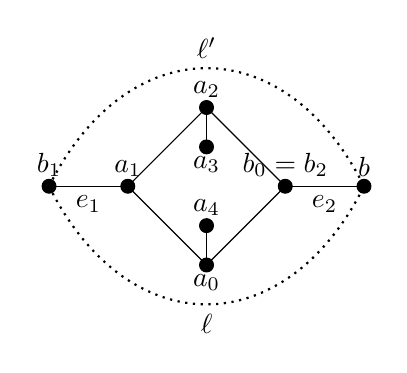
\begin{tikzpicture}[scale=0.5]
  \filldraw [black] (0,2) circle (5pt);
  \node [above] at (0,2) {$a_2$};
  \filldraw [black] (0,-2) circle (5pt);
  \node [below] at (0,-2) {$a_0$};
  \filldraw [black] (-2,0) circle (5pt);
  \node [above] at (-2,0) {$a_1$};
  \filldraw [black] (2,0) circle (5pt);
  \node [above] at (2,0) {$b_0=b_2$};
  \filldraw [black] (4,0) circle (5pt);
  \node [above] at (4,0) {$b$};
  \filldraw [black] (-4,0) circle (5pt);
  \node [above] at (-4,0) {$b_1$};

  \node[below] at (-3,0) {$e_1$};
  \node[below] at (3,0) {$e_2$};

  \filldraw [black] (0,1) circle (5pt);
  \node [below] at (0,1) {$a_3$};

  \filldraw [black] (0,-1) circle (5pt);
  \node [above] at (0,-1) {$a_4$};
  

  \draw (0,2) -- (2,0);
  \draw (2,0) -- (0,-2);
  \draw (0,-2) -- (-2,0);
  \draw (-2,0) -- (0,2);
  \draw(-2,0) -- (-4,0);
  \draw (2,0) -- (4,0);

  \draw (0,-1) -- (0,-2);
  \draw (0,1) -- (0,2);

  \draw[thick, dotted] (-4,0) .. controls (-2,4) and (2,4) ..(4,0);
  \draw[thick, dotted] (-4,0) .. controls (-2,-4) and (2,-4) .. (4,0);

  \node [above] at (0,3) {$\ell'$};
  \node [below] at (0,-3) {$\ell$};
  
  
  \end{tikzpicture}
  \captionsetup{justification=centering}
   \caption{When $b_0 = b_2$}
   \label{G-two-bounding-faces}
\end{figure}

We will now define two auxiliary graphs $G_1$ and $G_2$.
$G_1$ consists of the cycle $C$ and its interior 
region, augmented by a single edge $e^* = \{a_1, b_0\}$.
$G_2$ consists of everything in $G$ properly
exterior to the cycle $C$ (i.e.,
not containing $C$ and its interior)
with the two edges $e_1 =
\{a_1, b_1\}$ and $e_2 = \{b, b_0\}$ replaced by 
one new edge $e_{12} = \{a_1, b_0\}$. (See Figure~\ref{G1G2}). 
$G_1$ is not one of the exceptional graphs since it contains a pentagon.
If $G_2$ were $M_{2,3}$ then the two paths $\pi$ and $\pi'$
denoted by the dotted lines
with labels $\ell$ and $\ell'$  both consist of a single edge
and are present in $G$, contradicting $G$ being simple.
If $G_2$ were $K_4$ then there are four triangle faces (on the spherical embedding),
two of which must be present in $G$,  contradicting $G$ having
no triangle faces.
So, by induction, both $G_1$ and $G_2$
have a P3EM. Note that $G_1$ contains two
triangle faces separated by the edge $e^*$.
Any P3EM of $G_1$ assigns $e^*$ to one of these two
triangle faces which implies that all three edges
of this triangle face must be assigned to this face.
Thus, in Figure~\ref{G1}
% can you make ~\ref{G-two-bounding-faces}-2 for G2 sug-ref ?
the four edges $\{a_1, a_2\}, \{a_2, b_0\}, \{a_1, a_0\}, \{a_0, b_0\}$ must be assigned all up
or all down, according to whether $e^*$
is assigned down or up, respectively. 
In $G_2$, the edge $e_{12}$ is assigned either up or down
to the two adjacent faces. If $e_{12}$ is assigned up, then
along the path $\pi$ (resp. $\pi'$) of $\ell$ (resp. $\ell'$) 
edges there are
$0 \pmod 3$ (resp. $2 \pmod 3$) edges assigned toward the face
that $e_{12}$ is on its boundary.
If $e_{12}$ is assigned  down, then the opposite happens, i.e.,
$2 \pmod 3$ (resp. $0 \pmod 3$ ) edges of $\pi$ (resp. $\pi'$) 
 are assigned toward the  face that $e_{12}$ is on its boundary.

We now define an edge assignment  that will be a P3EM for $G$.
Every edge in $G$ other than $e_1$ and $e_2$ belongs to
exactly one of $G_1$ or $G_2$. We assign these edges according to
the assignment in  $G_1$ or $G_2$ respectively.
This satisfies the requirement of P3EM for every face other than
$\Delta$ and $\Delta'$ in $G$. For the
assignment on  $e_1$ and $e_2$, there are
four cases according to how $e^*$ in $G_1$ and $e_{12}$ in $G_2$
are assigned.
The first case is both $e^*$ in $G_1$  and $e_{12}$ in $G_2$ are
assign up, and we assign $e_1$ down and $e_2$ up in $G$.
Then,  there are a total of
3 edges $e_1 = \{b_1, a_1\}$,
$\{a_1, a_0\}$ and $\{a_0, b_0\}$ and $0 \pmod 3$  edges of $\pi$
assigned toward $\Delta$.
Also  there are a total of
1 edge $e_2 = \{b_0, b\}$,
and $2 \pmod 3$  edges of $\pi'$
assigned toward 
$\Delta'$.
The  second case is when $e^*$ and $e_{12}$  are assigned
respectively  up and down, and we assign $e_1$ and $e_2$ both
down in $G$. 
Then,  there are a total of
4 edges $e_1 = \{b_1, a_1\}$,
$\{a_1, a_0\}$, $\{a_0, b_0\}$  and $e_2 = (b_0, b)$,
and $2 \pmod 3$  edges of $\pi$
assigned toward $\Delta$, making it $0 \pmod 3$ altogether.
Also  there are no edge among these four
and  $0 \pmod 3$  edges of $\pi'$
assigned toward 
$\Delta'$. The other two cases are similar.
% really  symmetric. but i don't want to say that, because inside square
% and outside \pi \pi', things are actually not excatly symmeric
% but as far as the argument for the two Delta faces , really symmetric.
We have proved that a P3EM exists for $G$.

Hence we may assume that $b_0, \ldots, b_4$ are all distinct.

% Hi Professor, could you please look at my e-mail about revising figure 10? Thanks!
% OK 
% which do you want me to look?



\begin{figure}[ht]
  \centering
  \begin{subfigure}[b]{0.4\textwidth}
  \centering
  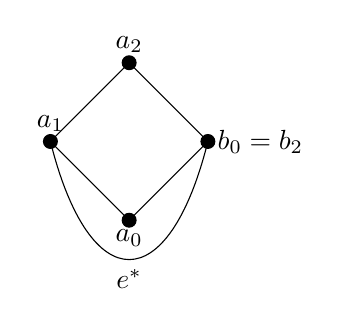
\begin{tikzpicture}[scale=0.5]
  \filldraw [black] (0,2) circle (5pt);
  \node [above] at (0,2) {$a_2$};
  \filldraw [black] (0,-2) circle (5pt);
  \node [below] at (0,-2) {$a_0$};
  \filldraw [black] (-2,0) circle (5pt);
  \node [above] at (-2,0) {$a_1$};
  \filldraw [black] (2,0) circle (5pt);
  \node [right] at (2,0) {$b_0=b_2$};
  

  \draw (0,2) -- (2,0);
  \draw (2,0) -- (0,-2);
  \draw (0,-2) -- (-2,0);
  \draw (-2,0) -- (0,2);
  \draw (-2,0) .. controls (-1,-4) and (1,-4) .. (2,0);

  \node [below] at (0,-3) {$e^*$};
  \end{tikzpicture}
  \captionsetup{justification=centering}
  \caption{$G_1$}
  \label{G1}
  \end{subfigure}
  \begin{subfigure}[b]{0.4\textwidth}
  \centering
  \begin{tikzpicture}[scale=0.5]
  \filldraw [black] (4,0) circle (5pt);
  \node [above] at (4,0) {$b$};
  \filldraw [black] (-4,0) circle (5pt);
  \node [above] at (-4,0) {$b_1$};
  \draw(-4,0) -- (4,0);
  \draw[thick, dotted] (-4,0) .. controls (-2,4) and (2,4) ..(4,0);
  \draw[thick, dotted] (-4,0) .. controls (-2,-4) and (2,-4) .. (4,0);
  \node [above] at (0,0) {$e_{12}$};
  \node [above] at (0,3) {$l'$};
  \node [below] at (0,-3) {$l$};
  \end{tikzpicture}
  \captionsetup{justification=centering}
  \caption{$G_2$}
  \label{G2}
  \end{subfigure}
  \captionsetup{justification=centering}
  \caption{$G_1$ and $G_2$}
  \label{G1G2}
\end{figure}



We claim that  there is a simple path connecting $b_i$ and $b_{i+1}$ for each $0 \leq i \leq 4$ (where $b_5 = b_0$), and furthermore
the cycle $(a_i, b_i, \ldots, b_{i+1}, a_{i+1}, a_i)$ using this path
is the  boundary of a face.
Define an $a_i$-R path as follows: start from $a_i$ and take the first edge  $\{a_i, b_i\}$, and then at every new vertex (of degree 3) choose
the right branch for the next vertex, until we encounter 
a previously visited vertex on this walk, or  one of $\{a_0, a_1 , \ldots, a_4\}$, then stop. For notational simplicity we 
consider the case for $i=0$;  all other cases are the same. Suppose the $a_0$-R path is $\{x_0, x_1, ..., x_k, ..., x_m\}$, where $x_0 = a_0$ and $ x_1 = b_0$.
First we claim $x_m  \neq a_0$.  If it were, then the step before would have been $a_1, a_4$ or $b_1 =x_0$, but then  the $a_0$-R path should have stopped at $x_{m-1}$. Next we claim that $x_m \in \{a_1,a_2,a_3,a_4\}$.
Indeed, if $x_m \not \in  \{a_1,a_2,a_3,a_4\}$, then it is a 
previously visited vertex $x_k$ on this walk, with $k \ge 1$.
Then $x_{k-1}$ exists.
Moreover,  $(x_k, x_{k+1}, \dots, x_m)$ is a cycle which is formed by
always taking the right branch at the next vertex. The last edge $(x_{m-1}, x_m)$ (which is $(x_{m-1}, x_k)$)
must be the left branch edge when coming from the direction $(x_{k-1}, x_k)$,
thus the traversal of the cycle  $(x_k, x_{k+1}, \dots, x_m)$ is counterclockwise.
%%% b/c two edges incident to x_k had been taken.
Thus 
 the edge $\{x_{k-1}, x_k\}$ is a bridge, a contradiction.
 See Figure~\ref{fig:simple paths between b_i's} for an illustration.

 \begin{figure}[ht]
  \centering
  \begin{tikzpicture}
  \filldraw [black] (0,0) circle (1pt);
  \node[left] at (0,0) {$a_0 = x_0$};
  \filldraw [black] (0,1) circle (1pt);
  \node[left] at (0,1) {$b_0 = x_1$};
  \draw (0,0) -- (0,1);

  \filldraw [black] (0.75,1.75) circle (1pt);
  \node[left] at (0.75,1.75) {$x_2$};
  \draw (0,1) -- (0.75,1.75);

  \draw (0,1) -- (-0.75,1.75);
  \draw (0.75,1.75) -- (0.5,2.25);
  \draw[thick, dotted] (0.75,1.75) -- (3,3);
  \draw[very thick] (3,3) -- (4,4);
  \draw (3,3) -- (2,3.5);
  \filldraw [black] (3,3) circle (1pt);
  \node[below] at (3,3) {$x_{k-1}$};
  \node[above left] at (4,4) {$x_k=x_m$};
  \draw (4,4) -- (4.5,3.5);
  \draw (4,4) -- (4.5,4.5);
  \filldraw [black] (4,4) circle (1pt);
  \filldraw [black] (4.5,3.5) circle (1pt);
  \filldraw [black] (4.5,4.5) circle (1pt);
  \node[above] at (4.5,4.5) {$x_{m-1}$};
  \node[below] at (4.5,3.5) {$x_{k+1}$};
  \draw[thick, dotted] (4.5,4.5) .. controls (6,5) and (6,3) .. (4.5,3.5);
  \draw (4.5,4.5) -- (5,4.25);
  \draw (4.5,3.5) -- (5,3.75);
  \draw (5.5,3.7) -- (5,3.85);
  \draw (5.5,4.3) -- (5,4);
  \filldraw [black] (5.5,3.7) circle (1pt);
  \filldraw [black] (5.5,4.3) circle (1pt);
  \end{tikzpicture}
  \captionsetup{justification=centering}
   \caption{Simple paths between $b_i$'s}
   \label{fig:simple paths between b_i's}
\end{figure}
 
 Next we claim that $x_m = a_1$, and $x_{m-1} = b_1$, (see  Figure~\ref{pentagon_path_1}).
 We prove this by eliminating the possibilities
 $x_m \in \{a_2, a_3, a_4\}$. Suppose  $x_m = a_4$. It follows from the definition 
 %As this is the first time stopping . by definition of stopping
 of the $a_0$-R path that
 $x_{m-1} \not \in \{a_0, a_1, \ldots, a_4\}$,
 being the step before $x_m$, and then the only way to reach $x_m = a_4$
is $x_{m-1} = b_4$. Since this  $a_0$-R path always  takes the
right branch, viewing the plane graph on a spherical embedding we can 
consider the face to the right of this  $a_0$-R path
as the outer face and then the edge $\{a_0, a_4\}$ is a chord.
However, by our assumption $G$ is chordless. 
Now suppose $x_m = a_3$. Then consider the $a_2$-R path.
By planarity and the fact that one single face
borders the right hand side of the 
{$a_0$-R}
path which ends in $a_3$,
the $a_2$-R path cannot end in $a_4$, and therefore
it must end in $a_1$. However, considering the indices mod 5 this is exactly the same
situation with the  $a_0$-R path ending in $a_4$, another contradiction.
Finally,  if the    $a_0$-R path ends in  $x_m = a_2$, then the
 $a_1$-R path would violate planarity, or produce a bridge. 
We conclude that  $x_m = a_1$. And then 
 it follows that $x_{m-1} = b_1$, and we have
 a face with boundary $(a_0, b_0, \ldots, b_1, a_1, a_0)$ 
 from this $a_0$-R path.
 The same is true for all $a_i$-R paths. 

 In other words, we now have a pentagon face $P$ depicted as in Figure~\ref{fig:final pentagon}.

 \begin{figure}[ht]
  \centering
%  \begin{subfigure}[b]{0.4\textwidth}
%  \centering
  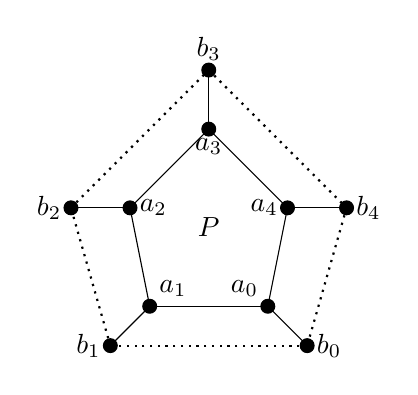
\begin{tikzpicture}[scale=0.5]
  \node at (0,0.5) {$P$};
  \filldraw [black] (1.5,-1.5) circle (5pt);
  \node[above left] at (1.5,-1.5) {$a_0$};
  \filldraw [black] (-1.5,-1.5) circle (5pt);
  \node[above right] at (-1.5,-1.5) {$a_1$};
  \filldraw [black] (-2,1) circle (5pt);
  \node[right] at (-2,1) {$a_2$};
  \filldraw [black] (2,1) circle (5pt);
  \node[left] at (2,1) {$a_4$};
  \filldraw [black] (0,3) circle (5pt);
  \node[below] at (0,3) {$a_3$};
  \filldraw [black] (2.5,-2.5) circle (5pt);
  \node[right] at (2.5,-2.5) {$b_0$};
  \filldraw [black] (-2.5,-2.5) circle (5pt);
  \node[left] at (-2.5,-2.5) {$b_1$};
  \filldraw [black] (-3.5,1) circle (5pt);
  \node[left] at (-3.5,1) {$b_2$};
  \filldraw [black] (3.5,1) circle (5pt);
  \node[right] at (3.5,1) {$b_4$};
  \filldraw [black] (0,4.5) circle (5pt);
  \node[above] at (0,4.5) {$b_3$};
  \draw (1.5,-1.5) -- (-1.5,-1.5);
  \draw (-1.5, -1.5) -- (-2,1);
  \draw (-2,1) -- (0,3);
  \draw (0,3) -- (2,1);
  \draw (2,1) -- (1.5,-1.5);
  \draw (1.5,-1.5) -- (2.5,-2.5);
  \draw (-1.5,-1.5) -- (-2.5,-2.5);
  \draw (0,3) -- (0,4.5);
  \draw (-2,1) -- (-3.5,1);
  \draw (2,1) -- (3.5,1);
  \draw[thick, dotted] (2.5,-2.5) -- (-2.5,-2.5);
  \draw[thick, dotted] (-2.5,-2.5) -- (-3.5,1);
  \draw[thick, dotted] (-3.5,1) -- (0,4.5);
  \draw[thick, dotted] (0,4.5) -- (3.5,1);
  \draw[thick, dotted] (3.5,1) -- (2.5,-2.5);
  \end{tikzpicture}  
  \captionsetup{justification=centering}
   \caption{Pentagon in the original graph}
   \label{fig:final pentagon}
\end{figure}



% \begin{figure}[t!]
%   \centering
%   \begin{subfigure}[b]{0.5\textwidth}
%   \centering
%   \begin{tikzpicture}[scale=0.45]
%   \filldraw [black] (1.5,-1.5) circle (5pt);
%   \node[above left] at (1.5,-1.5) {$a_0$};
%   \filldraw [black] (-1.5,-1.5) circle (5pt);
%   \node[above right] at (-1.5,-1.5) {$a_1$};
%   \filldraw [black] (-2,1) circle (5pt);
%   \node[right] at (-2,1) {$a_2$};
%   \filldraw [black] (2,1) circle (5pt);
%   \node[left] at (2,1) {$a_4$};
%   \filldraw [black] (0,3) circle (5pt);
%   \node[below] at (0,3) {$a_3$};
%   \filldraw [black] (3.5,-3.5) circle (5pt);
%   \node[right] at (3.5,-3.5) {$b_0$};
%   \filldraw [black] (-3.5,-3.5) circle (5pt);
%   \node[left] at (-3.5,-3.5) {$b_1$};
%   \filldraw [black] (-4.5,1) circle (5pt);
%   \node[left] at (-4.5,1) {$b_2$};
%   \filldraw [black] (4.5,1) circle (5pt);
%   \node[right] at (4.5,1) {$b_4$};
%   \filldraw [black] (0,5.5) circle (5pt);
%   \node[above] at (0,5.5) {$b_3$};
%   \draw (1.5,-1.5) -- (-1.5,-1.5);
%   \draw (-1.5, -1.5) -- (-2,1);
%   \draw (-2,1) -- (0,3);
%   \draw (0,3) -- (2,1);
%   \draw (2,1) -- (1.5,-1.5);
%   \draw (1.5,-1.5) -- (3.5,-3.5);
%   \draw (-1.5,-1.5) -- (-3.5,-3.5);
%   \draw (0,3) -- (0,5.5);
%   \draw (-2,1) -- (-4.5,1);
%   \draw (2,1) -- (4.5,1);
%   \draw[thick, dotted] (3.5,-3.5) .. controls (2,-5) and (-2,-5) .. (-3.5,-3.5);
%   \draw[thick, dotted] (-3.5,-3.5) .. controls (-5,-3) and (-6,-1).. (-4.5,1);
%   \draw[thick, dotted] (-4.5,1) .. controls (-6,4) and (-2,7) .. (0,5.5);
%   \draw[thick, dotted] (4.5,1) .. controls (6,4) and (2,7) .. (0,5.5);
%   \draw[thick, dotted] (3.5,-3.5) .. controls (5,-3) and (6,-1) .. (4.5,1); 
%   \draw[->, line width=0.3mm] (2.5, -2.5) -- (1.5,-3.5);
%   \draw[->, line width=0.3mm] (-2.5,-2.5) -- (-3.5,-1.5);
%   \draw[->, line width=0.3mm] (-3.25,1) -- (-3.25,2.55);
%   \draw[->, line width=0.3mm] (0,4) -- (1.5,4);
%   \draw[->, line width=0.3mm] (3.25,1) -- (3.25,-0.25);
%   \node at (2.5,-3.5) {$x_0$};
%   \node at (-3.25,-2.5) {$x_1$};
%   \node at (-3.75,1.75) {$x_2$};
%   \node at (0.75,4.5) {$x_3$};
%   \node at (4,0.25) {$x_4$};
%   \draw[->, line width=0.3mm] (0,-1.5) -- (0,-3);
%   \draw[->, line width=0.3mm] (-1.75,-0.25) -- (-3,-0.5);
%   \draw[->, line width=0.3mm] (1.75,-0.25) -- (3,-0.5);
%   \draw[->, line width=0.3mm] (-1.25,1.75) -- (-2.25,2.75);
%   \draw[->, line width=0.3mm] (1,2) -- (2,3);
%   \node at (-0.5,-2.25) {$y_0$};
%   \node at (-2.5,0) {$y_1$};
%   \node at (-1.25,2.5) {$y_2$};
%   \node at (2,2.25) {$y_3$};
%   \node at (2.25,-0.75) {$y_4$};
%   \draw[->, line width=0.3mm] (0,-4.5) -- (0,-6);
%   \draw[->, line width=0.3mm] (-5,-1) -- (-6.75,-1.25);
%   \draw[->, line width=0.3mm] (5,-1) -- (6.75,-1.25);
%   \draw[->, line width=0.3mm] (-4.25,4.25) -- (-5.5,5.5);
%   \draw[->, line width=0.3mm] (4.25,4.25) -- (5.5,5.5);
%   \node at (-0.5,-5.25) {$z_0$};
%   \node at (-5.75,-0.75) {$z_1$};
%   \node at (6,-1.5) {$z_4$};
%   \node at (-4.5,5.25) {$z_2$};
%   \node at (5.25,4.5) {$z_3$};
%   \end{tikzpicture}
%   \caption{pentagon in the original graph}
%   \label{pentagon_1}
%   \end{subfigure}
%   \begin{subfigure}[b]{0.45\textwidth}
%   \centering
%   \begin{tikzpicture}[scale=0.45]
%   \filldraw [black] (1.5,-1.5) circle (5pt);
%   \node[above left] at (1.5,-1.5) {$a_0$};
%   \filldraw [black] (2,1) circle (5pt);
%   \node[left] at (2,1) {$a_4$};
%   \filldraw [black] (0,3) circle (5pt);
%   \node[below] at (0,3) {$a_3$};
%   \filldraw [black] (3.5,-3.5) circle (5pt);
%   \node[right] at (3.5,-3.5) {$b_0$};
%   \filldraw [black] (-3.5,-3.5) circle (5pt);
%   \node[left] at (-3.5,-3.5) {$b_1$};
%   \filldraw [black] (-4.5,1) circle (5pt);
%   \node[left] at (-4.5,1) {$b_2$};
%   \filldraw [black] (4.5,1) circle (5pt);
%   \node[right] at (4.5,1) {$b_4$};
%   \filldraw [black] (0,5.5) circle (5pt);
%   \node[above] at (0,5.5) {$b_3$};
%   \draw (0,3) -- (2,1);
%   \draw (2,1) -- (1.5,-1.5);
%   \draw (1.5,-1.5) -- (3.5,-3.5);
%   \draw (0,3) -- (0,5.5);
%   \draw (2,1) -- (4.5,1);
%   \draw[thick, dotted] (3.5,-3.5) .. controls (2,-5) and (-2,-5) .. (-3.5,-3.5);
%   \draw[thick, dotted] (-3.5,-3.5) .. controls (-5,-3) and (-6,-1).. (-4.5,1);
%   \draw[thick, dotted] (-4.5,1) .. controls (-6,4) and (-2,7) .. (0,5.5);
%   \draw[thick, dotted] (4.5,1) .. controls (6,4) and (2,7) .. (0,5.5);
%   \draw[thick, dotted] (3.5,-3.5) .. controls (5,-3) and (6,-1) .. (4.5,1); 
%   \draw (-3.5,-3.5) -- (1.5,-1.5); % b_1 -- a_0
%   \draw (-4.5,1) -- (0,3); % b_2 -- a_3
%   \draw[->, line width=0.3mm] (2.5, -2.5) -- (1.5,-3.5);
%   \draw[->, line width=0.3mm] (0,4) -- (1.5,4);
%   \draw[->, line width=0.3mm] (3.25,1) -- (3.25,-0.25);
%   \draw[->, line width=0.3mm] (-1,-2.5) -- (-1.5,-1.25); % x'_1
%   \draw[->, line width=0.3mm] (-2.25,2) -- (-2.75,3.25); % x'_2
%   \node at (2.5,-3.35) {$x'_0$};
%   \node at (-2,-2.25) {$x'_1$};
%   \node at (-3.25,2.25) {$x'_2$};
%   \node at (0.75,4.65) {$x'_3$};
%   \node at (4,0.25) {$x'_4$};
%   \draw[->, line width=0.3mm] (1.75,-0.25) -- (3,-0.5);
%   \draw[->, line width=0.3mm] (1,2) -- (2,3);
%   \node at (2,2.25) {$y'_3$};
%   \node at (2.25,-1) {$y'_4$};
%   \draw[->, line width=0.3mm] (0,-4.5) -- (0,-6);
%   \draw[->, line width=0.3mm] (-5,-1) -- (-6.75,-1.25);
%   \draw[->, line width=0.3mm] (5,-1) -- (6.75,-1.25);
%   \draw[->, line width=0.3mm] (-4.25,4.25) -- (-5.5,5.5);
%   \draw[->, line width=0.3mm] (4.25,4.25) -- (5.5,5.5);
%   \node at (-0.5,-5.25) {$z'_0$};
%   \node at (-5.75,-0.5) {$z'_1$};
%   \node at (6,-1.75) {$z'_4$};
%   \node at (-4.5,5.25) {$z'_2$};
%   \node at (5.25,4.5) {$z'_3$};
%   \end{tikzpicture}
%   \caption{resulting graph}
%   \label{pentagon_2}
%   \end{subfigure}
%   \caption{Transforming a pentagon}
%   \label{pentagon}
% \end{figure}


\begin{figure}[ht]
  \centering
  \begin{subfigure}[b]{0.5\textwidth}
  \centering
  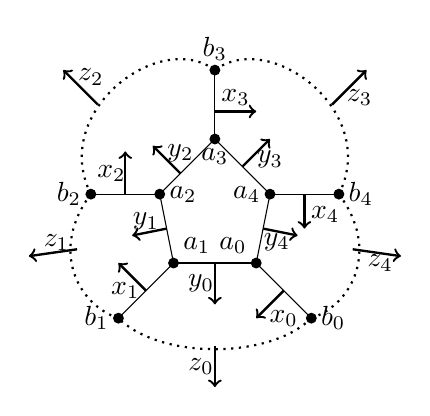
\begin{tikzpicture}[scale=0.35]
  \filldraw [black] (1.5,-1.5) circle (5pt);
  \node[above left] at (1.5,-1.5) {$a_0$};
  \filldraw [black] (-1.5,-1.5) circle (5pt);
  \node[above right] at (-1.5,-1.5) {$a_1$};
  \filldraw [black] (-2,1) circle (5pt);
  \node[right] at (-2,1) {$a_2$};
  \filldraw [black] (2,1) circle (5pt);
  \node[left] at (2,1) {$a_4$};
  \filldraw [black] (0,3) circle (5pt);
  \node[below] at (0,3) {$a_3$};
  \filldraw [black] (3.5,-3.5) circle (5pt);
  \node[right] at (3.5,-3.5) {$b_0$};
  \filldraw [black] (-3.5,-3.5) circle (5pt);
  \node[left] at (-3.5,-3.5) {$b_1$};
  \filldraw [black] (-4.5,1) circle (5pt);
  \node[left] at (-4.5,1) {$b_2$};
  \filldraw [black] (4.5,1) circle (5pt);
  \node[right] at (4.5,1) {$b_4$};
  \filldraw [black] (0,5.5) circle (5pt);
  \node[above] at (0,5.5) {$b_3$};
  \draw (1.5,-1.5) -- (-1.5,-1.5);
  \draw (-1.5, -1.5) -- (-2,1);
  \draw (-2,1) -- (0,3);
  \draw (0,3) -- (2,1);
  \draw (2,1) -- (1.5,-1.5);
  \draw (1.5,-1.5) -- (3.5,-3.5);
  \draw (-1.5,-1.5) -- (-3.5,-3.5);
  \draw (0,3) -- (0,5.5);
  \draw (-2,1) -- (-4.5,1);
  \draw (2,1) -- (4.5,1);
  \draw[thick, dotted] (3.5,-3.5) .. controls (2,-5) and (-2,-5) .. (-3.5,-3.5);
  \draw[thick, dotted] (-3.5,-3.5) .. controls (-5,-3) and (-6,-1).. (-4.5,1);
  \draw[thick, dotted] (-4.5,1) .. controls (-6,4) and (-2,7) .. (0,5.5);
  \draw[thick, dotted] (4.5,1) .. controls (6,4) and (2,7) .. (0,5.5);
  \draw[thick, dotted] (3.5,-3.5) .. controls (5,-3) and (6,-1) .. (4.5,1); 
  \draw[->, line width=0.3mm] (2.5, -2.5) -- (1.5,-3.5);
  \draw[->, line width=0.3mm] (-2.5,-2.5) -- (-3.5,-1.5);
  \draw[->, line width=0.3mm] (-3.25,1) -- (-3.25,2.55);
  \draw[->, line width=0.3mm] (0,4) -- (1.5,4);
  \draw[->, line width=0.3mm] (3.25,1) -- (3.25,-0.25);
  \node at (2.5,-3.5) {$x_0$};
  \node at (-3.25,-2.5) {$x_1$};
  \node at (-3.75,1.75) {$x_2$};
  \node at (0.75,4.5) {$x_3$};
  \node at (4,0.25) {$x_4$};
  \draw[->, line width=0.3mm] (0,-1.5) -- (0,-3);
  \draw[->, line width=0.3mm] (-1.75,-0.25) -- (-3,-0.5);
  \draw[->, line width=0.3mm] (1.75,-0.25) -- (3,-0.5);
  \draw[->, line width=0.3mm] (-1.25,1.75) -- (-2.25,2.75);
  \draw[->, line width=0.3mm] (1,2) -- (2,3);
  \node at (-0.5,-2.25) {$y_0$};
  \node at (-2.5,0) {$y_1$};
  \node at (-1.25,2.5) {$y_2$};
  \node at (2,2.25) {$y_3$};
  \node at (2.25,-0.75) {$y_4$};
  \draw[->, line width=0.3mm] (0,-4.5) -- (0,-6);
  \draw[->, line width=0.3mm] (-5,-1) -- (-6.75,-1.25);
  \draw[->, line width=0.3mm] (5,-1) -- (6.75,-1.25);
  \draw[->, line width=0.3mm] (-4.25,4.25) -- (-5.5,5.5);
  \draw[->, line width=0.3mm] (4.25,4.25) -- (5.5,5.5);
  \node at (-0.5,-5.25) {$z_0$};
  \node at (-5.75,-0.75) {$z_1$};
  \node at (6,-1.5) {$z_4$};
  \node at (-4.5,5.25) {$z_2$};
  \node at (5.25,4.5) {$z_3$};
  \end{tikzpicture}
  \captionsetup{justification=centering}
  \caption{pentagon in the original graph}
  \label{pentagon_1}
  \end{subfigure}
  \begin{subfigure}[b]{0.45\textwidth}
  \centering
  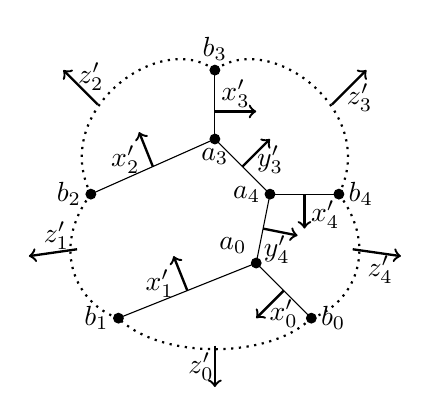
\begin{tikzpicture}[scale=0.35]
  \filldraw [black] (1.5,-1.5) circle (5pt);
  \node[above left] at (1.5,-1.5) {$a_0$};
  \filldraw [black] (2,1) circle (5pt);
  \node[left] at (2,1) {$a_4$};
  \filldraw [black] (0,3) circle (5pt);
  \node[below] at (0,3) {$a_3$};
  \filldraw [black] (3.5,-3.5) circle (5pt);
  \node[right] at (3.5,-3.5) {$b_0$};
  \filldraw [black] (-3.5,-3.5) circle (5pt);
  \node[left] at (-3.5,-3.5) {$b_1$};
  \filldraw [black] (-4.5,1) circle (5pt);
  \node[left] at (-4.5,1) {$b_2$};
  \filldraw [black] (4.5,1) circle (5pt);
  \node[right] at (4.5,1) {$b_4$};
  \filldraw [black] (0,5.5) circle (5pt);
  \node[above] at (0,5.5) {$b_3$};
  \draw (0,3) -- (2,1);
  \draw (2,1) -- (1.5,-1.5);
  \draw (1.5,-1.5) -- (3.5,-3.5);
  \draw (0,3) -- (0,5.5);
  \draw (2,1) -- (4.5,1);
  \draw[thick, dotted] (3.5,-3.5) .. controls (2,-5) and (-2,-5) .. (-3.5,-3.5);
  \draw[thick, dotted] (-3.5,-3.5) .. controls (-5,-3) and (-6,-1).. (-4.5,1);
  \draw[thick, dotted] (-4.5,1) .. controls (-6,4) and (-2,7) .. (0,5.5);
  \draw[thick, dotted] (4.5,1) .. controls (6,4) and (2,7) .. (0,5.5);
  \draw[thick, dotted] (3.5,-3.5) .. controls (5,-3) and (6,-1) .. (4.5,1); 
  \draw (-3.5,-3.5) -- (1.5,-1.5); % b_1 -- a_0
  \draw (-4.5,1) -- (0,3); % b_2 -- a_3
  \draw[->, line width=0.3mm] (2.5, -2.5) -- (1.5,-3.5);
  \draw[->, line width=0.3mm] (0,4) -- (1.5,4);
  \draw[->, line width=0.3mm] (3.25,1) -- (3.25,-0.25);
  \draw[->, line width=0.3mm] (-1,-2.5) -- (-1.5,-1.25); % x'_1
  \draw[->, line width=0.3mm] (-2.25,2) -- (-2.75,3.25); % x'_2
  \node at (2.5,-3.35) {$x'_0$};
  \node at (-2,-2.25) {$x'_1$};
  \node at (-3.25,2.25) {$x'_2$};
  \node at (0.75,4.65) {$x'_3$};
  \node at (4,0.25) {$x'_4$};
  \draw[->, line width=0.3mm] (1.75,-0.25) -- (3,-0.5);
  \draw[->, line width=0.3mm] (1,2) -- (2,3);
  \node at (2,2.25) {$y'_3$};
  \node at (2.25,-1) {$y'_4$};
  \draw[->, line width=0.3mm] (0,-4.5) -- (0,-6);
  \draw[->, line width=0.3mm] (-5,-1) -- (-6.75,-1.25);
  \draw[->, line width=0.3mm] (5,-1) -- (6.75,-1.25);
  \draw[->, line width=0.3mm] (-4.25,4.25) -- (-5.5,5.5);
  \draw[->, line width=0.3mm] (4.25,4.25) -- (5.5,5.5);
  \node at (-0.5,-5.25) {$z'_0$};
  \node at (-5.75,-0.5) {$z'_1$};
  \node at (6,-1.75) {$z'_4$};
  \node at (-4.5,5.25) {$z'_2$};
  \node at (5.25,4.5) {$z'_3$};
  \end{tikzpicture}
  \captionsetup{justification=centering}
  \caption{resulting graph}
  \label{pentagon_2}
  \end{subfigure}
  \captionsetup{justification=centering}
  \caption{Transforming a pentagon}
  \label{pentagon}
\end{figure}
We now perform the transformation as illustrated in Figure~\ref{pentagon}. 
The transformed graph ({\bf b}) on the right is not $M_{2,3}$ or $K_4$
by vertex count. By induction there is a P3EM $M'$ on the transformed graph.
We use  Boolean variables $x'_i$ ($0 \leq i \leq 4$), 
and $y'_3$, $y'_4$ to denote the assignment on those 7 edges in Figure~\ref{pentagon}b, 
such that the variable is  1 
 if the  corresponding  edge is assigned to the face indicated by its arrow, and is 0 if 
 it is assigned to the face on the other side.
 We also use
nonnegative integer
 variables $z'_i$ ($0 \leq i \leq 4$) to denote the number  of edges
 assigned to the  side indicated along the simple path $b_i$ to $b_{i+1}$.
Now we define a P3EM $M$ on $G$ using $M'$ as follows.
 All edges in $G$ that are not incident to $a_0, a_1, a_2, a_3$ or $a_4$ 
 will retain their assignment as in $M'$. These include all edges
 on the path $b_i$ to $b_{i+1}$ (and all edges beyond these simple paths that are not
 depicted in Figure~\ref{pentagon}a.)
 In particular, if $z_i$ ($0 \leq i \leq 4$) is the number  of edges
 assigned to the  side indicated along the simple path $b_i$ to $b_{i+1}$ in $G$,
 then $z_i = z'_i$.
For the 10 edges incident to at least one of $a_0, a_1, a_2, a_3$ or $a_4$ in Figure~\ref{pentagon}a we will use  Boolean variables $x_i$ and $y_i$ ($0 \leq i \leq 4$) to denote
the  assignment of $M$ on $G$, such that the variable is  1 
 if the  corresponding  edge is assigned to the face indicated by its arrow, and is 0 
 otherwise.
 
 A moment's reflection will convince the reader that
 $M$ is a P3EM on $G$ iff we can assign Boolean 0-1 variables 
 $x_i$ and $y_i$ ($0 \leq i \leq 4$) that satisfy the following equation system $(\Sigma)$,
 where $\overline{x} = 1- x \in \{0, 1\}$ denotes the negation of
 the  Boolean variable  $x$.
{\small
\begin{empheq}[left=(\Sigma)~~~\empheqlbrace]{align}
  &x_0 + y_0 + \overline{x_1} \equiv x'_0 + \overline{x'_1} \pmod{3} \notag
  \\
  &x_2 + y_2 + \overline{x_3} \equiv x'_2 + \overline{x'_3} \pmod{3} \notag
  \\
  &x_3 + y_3 + \overline{x_4} \equiv x'_3 + y'_3 + \overline{x'_4} \pmod{3} \notag
  \\
  &x_4 + y_4 + \overline{x_0} \equiv x'_4 + y'_4 + \overline{x'_0} \pmod{3} \notag
  \\
  &x_1 + y_1 + \overline{x_2} \equiv x'_1 + \overline{x'_2} + \overline{y'_3} + \overline{y'_4} \pmod{3} \notag
  \\
  &\sum\limits_{i=0}^{4} \overline{y_i} \equiv 0 \pmod{3} \notag
\end{empheq}
}

We note that, while this equation system consists of all linear equations
mod 3, it is not an ordinary linear equation system over $\mathbb{Z}_3$;
the complicating factor is that all the variables must take Boolean values in $\{0, 1\}$.
Somewhat miraculously, we show that for any Boolean values of
$x'_i$ ($0 \leq i \leq 4$) 
and $y'_3$, $y'_4$, we  can always solve the equation system $(\Sigma)$
for the Boolean variables 
 $x_i$ and $y_i$ ($0 \leq i \leq 4$). 
 
 If $(y'_3, y'_4) \neq (0,0)$, then we set $x_i = x'_i$ for $0 \leq i \leq 4$, $y_3 = y'_3$, $y_4 = y'_4$, $y_0=y_2 =0$,  and
$y_1 = \overline{y'_3} + \overline{y'_4} \in \{ 0, 1\}$. (Note that
 $(y'_3, y'_4) \neq (0,0)$ is used to obtain
$\overline{y'_3} + \overline{y'_4} \in \{ 0, 1\}$.)
One can check that this assignment
solves $(\Sigma)$.  

Now suppose $(y'_3, y'_4) = (0,0)$. The system of equations now becomes
{\small
\begin{empheq}[left=(\Sigma')~~~\empheqlbrace]{align}
  &x_0 + y_0 + \overline{x_1} \equiv x'_0 + \overline{x'_1} \pmod{3} \notag
  \\
  &x_2 + y_2 + \overline{x_3} \equiv x'_2 + \overline{x'_3} \pmod{3} \notag
  \\
  &x_3 + y_3 + \overline{x_4} \equiv x'_3 + \overline{x'_4} \pmod{3} \notag
  \\
  &x_4 + y_4 + \overline{x_0} \equiv x'_4 + \overline{x'_0} \pmod{3} \notag
  \\
  &x_1 + y_1 + \overline{x_2} \equiv x'_1 + \overline{x'_2} + 2 \pmod{3} \notag
  \\
  &\sum\limits_{i=0}^{4}  \overline{y_i} \equiv 0 \pmod{3} \notag
\end{empheq}
}

If $x'_1 = 0$, then we set $x_1 = 1$, and $x_i = x'_i$ for $0 \leq i \leq 4$, $i \neq 1$,
and set $y_2 = y_3 = y_4 = 0$, $y_0 = y_1 = 1$.
One can check that this assignment
solves  $(\Sigma')$. If $(x'_1, x'_2) = (1,1)$, then we set
$x_2 = 0$, and $x_i = x'_i$ for $0 \leq i \leq 4$,  $i \neq 2$, and set
$y_0 = y_3 = y_4 = 0$, $y_1 = y_2 = 1$. This  solves $(\Sigma')$. Thus it remains to consider the case when $(x'_1, x'_2) = (1,0)$. 
There remain eight cases, each corresponding to an assignment  
$(x'_0, x'_3, x'_4) \in \{0, 1\}^3$.

At this point we have $(y'_3, y'_4) = (0,0)$ in addition to $(x'_1, x'_2) = (1,0)$, so 
now we are  in a situation in Figure~\ref{pentagon}b where $x'_1, x'_2, y'_3$ and $y'_4$ are all pointing into the face bounded by the cycle $(b_1, a_0, a_4, a_3, b_2, \ldots, b_1)$. By 
a reflection along the $\{a_4,b_4\}$-axis, we only need to consider four cases,
with $x'_4 =0$.  These four cases are explicitly given in
Figure~\ref{geometry}, where we use a double arrow to indicate
an actual assignment of the corresponding edge into the face indicated.
For example, the following figure deals with the case  $(x'_0, x'_3 , x'_4) =(0, 0, 0)$.
\begin{figure}[H]
  \centering
  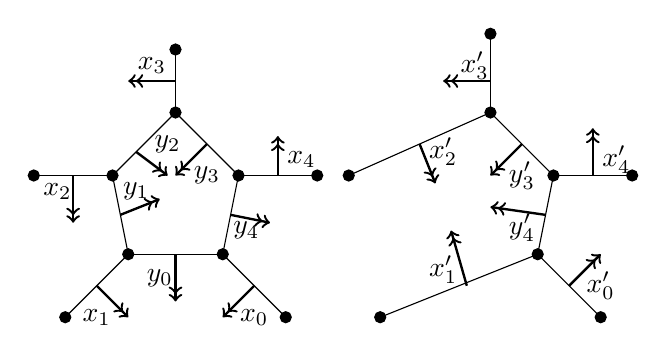
\begin{tikzpicture}[scale=0.4]
  \filldraw [black] (1.5,-1.5) circle (5pt);
%  \node[above left] at (1.5,-1.5) {$a_0$};
  \filldraw [black] (-1.5,-1.5) circle (5pt);
%  \node[above right] at (-1.5,-1.5) {$a_1$};
  \filldraw [black] (-2,1) circle (5pt);
%  \node[right] at (-2,1) {$a_2$};
  \filldraw [black] (2,1) circle (5pt);
%  \node[left] at (2,1) {$a_4$};
  \filldraw [black] (0,3) circle (5pt);
%  \node[below] at (0,3) {$a_3$};
  \filldraw [black] (3.5,-3.5) circle (5pt);
%  \node[right] at (3.5,-3.5) {$b_0$};
  \filldraw [black] (-3.5,-3.5) circle (5pt);
%  \node[left] at (-3.5,-3.5) {$b_1$};
  \filldraw [black] (-4.5,1) circle (5pt);
%  \node[left] at (-4.5,1) {$b_2$};
  \filldraw [black] (4.5,1) circle (5pt);
%  \node[right] at (4.5,1) {$b_4$};
  \filldraw [black] (0,5) circle (5pt);
%  \node[above] at (0,5.5) {$b_3$};
  \draw (1.5,-1.5) -- (-1.5,-1.5);
  \draw (-1.5, -1.5) -- (-2,1);
  \draw (-2,1) -- (0,3);
  \draw (0,3) -- (2,1);
  \draw (2,1) -- (1.5,-1.5);
  \draw (1.5,-1.5) -- (3.5,-3.5);
  \draw (-1.5,-1.5) -- (-3.5,-3.5);
  \draw (0,3) -- (0,5);
  \draw (-2,1) -- (-4.5,1);
  \draw (2,1) -- (4.5,1);
  \draw[->>, line width=0.3mm] (2.5, -2.5) -- (1.5,-3.5);
  \draw[->>, line width=0.3mm] (-2.5,-2.5) -- (-1.5,-3.5);
  \draw[->>, line width=0.3mm] (-3.25,1) -- (-3.25,-0.5);
  \draw[->>, line width=0.3mm] (0,4) -- (-1.5,4);
  \draw[->>, line width=0.3mm] (3.25,1) -- (3.25,2.25);
%  \node at (2.5,-3.5) {$x_0$};
%  \node at (-3.25,-2.5) {$x_1$};
%  \node at (-3.75,1.75) {$x_2$};
%  \node at (0.75,4.5) {$x_3$};
%  \node at (4,0.25) {$x_4$};
  \draw[->>, line width=0.3mm] (0,-1.5) -- (0,-3);
  \draw[->>, line width=0.3mm] (-1.75,-0.25) -- (-0.5,0.25);
  \draw[->>, line width=0.3mm] (1.75,-0.25) -- (3,-0.5);
  \draw[->>, line width=0.3mm] (-1.25,1.75) -- (-0.25,1);
  \draw[->>, line width=0.3mm] (1,2) -- (0,1);
  \node at (2.5,-3.5) {$x_0$};
  % \node at (-3.25,-2.5) {$x_1$};
  \node at (-2.5,-3.5) {$x_1$};
  % \node at (-3.75,1.75) {$x_2$};
  \node at (-3.75,0.5) {$x_2$};
  % \node at (0.75,4.5) {$x_3$};
  \node at (-0.75,4.5) {$x_3$};
  % \node at (4,0.25) {$x_4$};
  \node at (4,1.5) {$x_4$};
  \node at (-0.5,-2.25) {$y_0$};
  % \node at (-2.5,0) {$y_1$};
  \node at (-1.25,0.5) {$y_1$};
  % \node at (-1.25,2.5) {$y_2$};
  \node at (-0.25,2) {$y_2$};
  % \node at (2,2.25) {$y_3$};
  \node at (1,1) {$y_3$};
  \node at (2.25,-0.75) {$y_4$};
%  \node at (-0.5,-2.25) {$y_0$};
%  \node at (-2.5,0) {$y_1$};
%  \node at (-1.25,2.5) {$y_2$};
%  \node at (2,2.25) {$y_3$};
%  \node at (2.25,-0.75) {$y_4$};
  \filldraw [black] (11.5,-1.5) circle (5pt);
%  \node[above left] at (1.5,-1.5) {$a_0$};
  \filldraw [black] (12,1) circle (5pt);
%  \node[left] at (2,1) {$a_4$};
  \filldraw [black] (10,3) circle (5pt);
%  \node[below] at (0,3) {$a_3$};
  \filldraw [black] (13.5,-3.5) circle (5pt);
%  \node[right] at (3.5,-3.5) {$b_0$};
  \filldraw [black] (6.5,-3.5) circle (5pt);
%  \node[left] at (-3.5,-3.5) {$b_1$};
  \filldraw [black] (5.5,1) circle (5pt);
%  \node[left] at (-4.5,1) {$b_2$};
  \filldraw [black] (14.5,1) circle (5pt);
%  \node[right] at (4.5,1) {$b_4$};
  \filldraw [black] (10,5.5) circle (5pt);
%  \node[above] at (0,5.5) {$b_3$};
  \draw (10,3) -- (12,1);
  \draw (12,1) -- (11.5,-1.5);
  \draw (11.5,-1.5) -- (13.5,-3.5);
  \draw (10,3) -- (10,5.5);
  \draw (12,1) -- (14.5,1);
  \draw (6.5,-3.5) -- (11.5,-1.5); % b_1 -- a_0
  \draw (5.5,1) -- (10,3); % b_2 -- a_3
  \draw[->>, line width=0.3mm] (12.5, -2.5) -- (13.5,-1.5);
  \draw[->>, line width=0.3mm] (10,4) -- (8.5,4);
  \draw[->>, line width=0.3mm] (13.25,1) -- (13.25,2.5);
  \draw[->>, line width=0.3mm] (9.25,-2.5) -- (8.75,-0.75); % x'_1
  \draw[->>, line width=0.3mm] (7.75,2) -- (8.25,0.75); % x'_2
%  \node at (2.5,-3.35) {$x'_0$};
%  \node at (-2,-2.25) {$x'_1$};
%  \node at (-3.25,2.25) {$x'_2$};
%  \node at (0.75,4.65) {$x'_3$};
%  \node at (4,0.25) {$x'_4$};
  \draw[->>, line width=0.3mm] (11.75,-0.25) -- (10,0);
  \draw[->>, line width=0.3mm] (11,2) -- (10,1);
%  \node at (2,2.25) {$y'_3$};
%  \node at (2.25,-1) {$y'_4$};
  \node at (13.5,-2.5) {$x'_0$};
  \node at (8.5,-2) {$x'_1$};
  \node at (8.5,1.75) {$x'_2$};
  \node at (9.5,4.5) {$x'_3$};
  % \node at (4,0.25) {$x_4$};
  \node at (14,1.5) {$x'_4$};
  % \node at (2,2.25) {$y_3$};
  \node at (11,1) {$y'_3$};
  \node at (11,-0.65) {$y'_4$};
  \end{tikzpicture}
  \captionsetup{justification=centering}
  \caption{$(x'_0,x'_3,x'_4) = (0,0,0)$}
\label{fig:geometric inside proof}
\end{figure}

For other cases, see Figure~\ref{geometry}. 

Finally, we note that  the proof is constructive.
When smaller graphs are defined for induction purposes,
the size of the smaller graph strictly decreases
and in the case when two smaller graphs are needed (as in the case
dealing with a chord or getting distinct $b_i$'s) the sum of
sizes of the smaller graphs is approximately that of the original graph.
Tracing through the proof it can be easily verified that 
a planar 3-way edge
matching can be found in polynomial time.
This completes the proof of Theorem~\ref{thm:P3EM}.
\end{proof}